\documentclass[conference]{IEEEtran}
\IEEEoverridecommandlockouts
% The preceding line is only needed to identify funding in the first footnote. If that is unneeded, please comment it out.
\usepackage{cite}
\usepackage{amsmath,amssymb,amsfonts}

\usepackage{graphicx}
\usepackage[croatian]{babel}
\usepackage{textcomp}
\usepackage{xcolor}
\usepackage{tikz}
\usepackage[utf8]{inputenc}
\usepackage{verbatim}
\usetikzlibrary{arrows,shapes}
\usepackage{float}

\usepackage{algorithm}
\usepackage{algpseudocode}

\usepackage{pythonhighlight}

\usepackage{listings}
\lstset{basicstyle=\ttfamily,breaklines=true}



\renewcommand\IEEEkeywordsname{Ključne riječi}

\usepackage[utf8]{inputenc}
\usepackage{multicol}

\usepackage[bf, font=footnotesize]{caption}
% \usepackage[labelfont=small, font=small]{subcaption}


\makeatletter
\renewcommand{\ALG@name}{Algoritam}
\makeatother

\renewcommand{\lstlistingname}{Program}

\def\BibTeX{{\rm B\kern-.05em{\sc i\kern-.025em b}\kern-.08em
    T\kern-.1667em\lower.7ex\hbox{E}\kern-.125emX}}
\begin{document}
\pgfdeclarelayer{background}
\pgfsetlayers{background,main}
\long\def\/*#1*/{}

\title{Problem traženja minimalnog povezujućeg stabla\\
}

\author{\IEEEauthorblockN{Kerim Kadušić}
\IEEEauthorblockA{\textit{Elektrotehnički fakultet} \\
\textit{Univerzitet u Sarajevu}\\
Sarajevo, Bosna i Hercegovina \\
kkadusic1@etf.unsa.ba}
\and
\IEEEauthorblockN{Lino Bevanda}
\IEEEauthorblockA{\textit{Elektrotehnički fakultet} \\
\textit{Univerzitet u Sarajevu}\\
Sarajevo, Bosna i Hercegovina \\
lbevanda1@etf.unsa.ba}

% \and
% \IEEEauthorblockN{3\textsuperscript{rd} Given Name Surname}
% \IEEEauthorblockA{\textit{dept. name of organization (of Aff.)} \\
% \textit{name of organization (of Aff.)}\\
% City, Country \\
% email address or ORCID}
% \and
% \IEEEauthorblockN{4\textsuperscript{th} Given Name Surname}
% \IEEEauthorblockA{\textit{dept. name of organization (of Aff.)} \\
% \textit{name of organization (of Aff.)}\\
% City, Country \\
% email address or ORCID}
% \and
% \IEEEauthorblockN{5\textsuperscript{th} Given Name Surname}
% \IEEEauthorblockA{\textit{dept. name of organization (of Aff.)} \\
% \textit{name of organization (of Aff.)}\\
% City, Country \\
% email address or ORCID}
% \and
% \IEEEauthorblockN{6\textsuperscript{th} Given Name Surname}
% \IEEEauthorblockA{\textit{dept. name of organization (of Aff.)} \\
% \textit{name of organization (of Aff.)}\\
% City, Country \\
% email address or ORCID}
}

\maketitle

\begin{abstract}
U ovom radu je razmatran problem traženja minimalnog povezujućeg stabla uz objašnjenje osnovnh pojmova teorije grafova koji su relevatni za ovaj problem. Proučavane su metode i raspoloživi algoritmi, nakon čega se pristupilo detaljnoj analizi odabranog Primovog algoritma koja je bila potrebna za uspješnu implementaciju istog u programskog jeziku Python. Implementirani algoritam se potom primjenio na primjere problema praktične prirode što je omogućilo daljnju analizu principa traženja minimalnog povezujućeg stabla uz slikoviti prikaz svakog koraka algoritma. Na samom kraju testirane su performanse algoritma, te predložen način optimizacije istog.
\end{abstract}

\begin{IEEEkeywords}
Minimalno povezujuće stablo, Primov algoritam, graf, matrica susjedstva
\end{IEEEkeywords}

\section{Uvod}


S razvojem računarske nauke pojavljivali su se različiti problemi koji su se opisivali različitim  strukturama podataka. Među strukturama podataka su se posebno isticali grafovi koji svoju primjenu nemaju samo u računarstvu i informatici, nego i u drugim domenima poput matematike i elektrotehnike.
Snaga grafova se ogleda u mogućnosti objedinjavanja skupine objekata i njihovih relacija. Graf definišemo kao strukturu podataka koju čini skupina objekata (čvorovi) i koji su međusobno povezani relacijama ili vezama (grane grafa) \cite{b1}.

Za grafove se vežu uobičajeni problemi koji se korištenjem različitih algoritama uspješno rješavaju. Neki od poznatijih problema su navedeni u nastavku:

\begin{itemize}
    \item Otkrivanje najdužeg ili najkraćeg puta između dva čvora
    \item Pretraživanje grafova
    \item Problem maksimalnog protoka
    \item Problem traženja minimalnog povezujućeg stabla
    \item Uparivanje u grafovima
\end{itemize}

U fokusu razmatranja ovog rada će biti problem traženja minimalnog povezujućeg stabla. Prije upoznavanja s ovim problemom potrebno je definisati pojam stabla. Stablo predstavlja neusmjereni povezani aciklični graf, pri čemu neusmjereni grafovi predstavljaju grafove kod kojih je svaka veza između dva čvora $x$ i $y$ obostrana. Pod acikličnim grafovima se podrazumjevaju oni grafovi koji ne posjeduju cikluse \cite{b2}. Da bi neusmjereni povezani aciklični graf bio stablo mora ispuniti nekoliko uslova:

\begin{enumerate}
    \item Ako graf ima $n$ čvorova, onda on mora posjedovati $n-1$ grana
    \item Graf koji predstavlja stablo gubi svojstvo povezanosti ukoliko mu se ukloni bilo koja grana, odnosno u tom slučaju graf više nije stablo
    \item Ako se između svaka dva čvora grafa nalazi tačno jedan put koji ne prolazi više puta kroz isti čvor (elementarni put)
\end{enumerate}

Za navedene grafove koji ne ispunjavaju ove uslove vrijedi da su interno sadržani od barem jednog podgrafa koji ispunjava uslove tj. svaki povezani aciklični neusmjereni graf posjeduje barem jedno stablo. Takva stabla se nazivaju povezujućim stablima ili kosturima grafa \cite{b1}.

\tikzstyle{vertex}=[circle,fill=black!25,minimum size=20pt,inner sep=0pt]
\tikzstyle{selected vertex} = [vertex, fill=red!24]
\tikzstyle{edge} = [draw,thick,-]
\tikzstyle{weight} = [font=\small]
\tikzstyle{selected edge} = [draw,line width=5pt,-,red!50]
\tikzstyle{ignored edge} = [draw,line width=5pt,-,black!20]

\begin{figure}[H]
\begin{center}
\begin{tikzpicture}[scale=1.2, auto,swap]
    % Draw a 7,11 network
    % First we draw the vertices
    \foreach \pos/\name in {{(0,2)/a}, {(2,1)/b}, {(4,1)/c},
                            {(0,0)/d}, {(3,0)/e}, {(2,-1)/f}, {(4,-1)/g}}
        \node[vertex] (\name) at \pos {$\name$};
    % Connect vertices with edges and draw weights
    \foreach \source/ \dest /\weight in {b/a/7, c/b/8,d/a/5,d/b/9,
                                         e/b/7, e/c/5,e/d/15,
                                         f/d/6,f/e/8,
                                         g/e/9,g/f/11}
        \path[edge] (\source) -- node[weight] {$\weight$} (\dest);
 

\end{tikzpicture}
\caption{Primjer acikličnog neusmjerenog grafa}
\end{center}
\end{figure}

Na Slici 1. svakoj grani grafa je pridružena vrijednost. Ta vrijednost predstavlja težinu grane, te stoga prikazani graf predstavlja i težinski graf. Problem traženja minimalnog povezujućeg stabla se zasniva na pronalasku povezujućeg stabla tako da je zbir težina grana koje ga čine najmanji.

Ovaj problem se u praksi najčešće povezuje sa problemima povezivanja svih čvorova tako da se upotrijebi što manje resursa. Neka na primjer postoji ograničena dužina kablova koje je potrebno iskoristiti za povezivanje dalekovoda međusobno u elektrodistribucionu mrežu. Rješavanjem problema minimalnog povezujućeg stabla  moguće saznati minimalnu potrebnu dužinu kablova koja se treba iskoristiti za povezivanje dalekovoda. Generalno, uspješnim rješavanjem ovog problema postiže se tražena ušteda resursa.

Za problem rješavanja minimalnog povezujućeg stabla su razvijeni efikasni algoritmi. Među njima se posebno ističu Kruskalov i Primov algoritam. U nastavku će biti riječi o nekim poznatijim algoritmima za rješavanje problema minimalnog povezujućeg stabla.

\subsection{Borůvka algoritam}
Borůvka algoritam je prvi algoritam korišten u oblasti nalaženja minimalnog povezujućeg stabla.  Otkrio ga je 1926. godine češki matematičar Otakar Borůvka, tražeći efikasni način postavljanja električne mreže \cite{b3}.


\subsection{Kruskalov algoritam}
Kruskalov algoritam se obično primjenuje nad rijetkim grafovima. U prvoj iteraciji je potrebno uzeti granu koja ima najmanju težinu. Ukoliko postoji više grana sa istom težinom koja je ujedno i najmanja, svejedno je koja će biti odabrana. U narednim iteracijama je potrebno uzeti granu s najmanjom težinom od onih grana koje nisu do tada uzete, tako da ta grana ne obrazuje ciklus s do tada uzetim granama. Ovaj postupak se iterativno ponavlja sve dok se ne obrazuje povezujuće stablo \cite{b4}. 



% ---------------------------------------------------------------------------
% ------------------------ KORIŠTENI ALGORITAM ---------------------------
% ---------------------------------------------------------------------------

\section{Korišteni algoritam}
Za potrebe ovog rada implementiran je Primov algoritam. Primov algoritam je razvio češki matematičar Vojtěch Jarník 1930. godine koji je svoju popularnost stekao tek 30-ak godina kasnije, kada su Robert C. Prim i Edsger W. Dijkstra uvidjeli mogućnost primjene algoritma u računarskoj nauci i odlučili republicirati algoritam. Primov algoritam dolazi u različitim verzijama s obzirom da je osnovna verzija bila reda vremenske kompleksnosti $\mathcal{O}(n^3)$  gdje $n$ predstavlja broj čvorova grafa, što predstavlja lošiju vremensku kompleksnost od jednostavnijeg Kruskalovog algoritma reda $\mathcal{O}(m\log_2 m)$. Poboljšane verzije Primovog algoritma, osim bolje vremenske kompleksnosti, pogodnije su za primjenu kod gustih grafova u odnosu na druge algoritme \cite{b2}.

Bitno je napomenuti da Primov algoritam, kao i Borůvka i Kruskalov algoritam, spada u porodicu tzv. \textit{pohlepnih} ili \textit{proždrljivih} (engl. \textit{greedy}) algoritama, što znači da u svakom koraku vrši izbor one odluke koja u tom trenutku najviše doprinosi konačnom cilju, ne vodeći računa kako će se taj izbor odraziti na eventualne odluke koje će biti naknadno donesene. Generalno problem minimalno povezujućeg stabla ima izuzetno mnogo dopustivih rješenja koja ne moraju biti optimalna. Prema \textit{Cayleyevoj} teoremi iz teorije grafova, graf sa n čvorova može imati čak do $n^{n-2}$ povezujućih stabala \cite{b4}.


Osnova ideja rada Primovog algoritma je sljedeća: Za početak je potrebno odabrati proizvoljan čvor grafa te u kostur dodati granu s najmanjom težinom koja izlazi iz tog čvora. U narednoj iteraciji u stablo se dodaje grana sa najmanjom težinom od grana koje spajaju čvorove koji se trenutno nalaze u stablu s njima susjednim čvorovima koji još nisu ušli u stablo. Ovaj postupak se ponavlja sve dok se ne formira povezujuće stablo (kostur), odnosno sve dok se ne izabere $n-1$ grana (pri čemu je n broj čvorova grafa) \cite{b1}.

Dakle kod Primovog algoritma u svakoj iteraciji postoji stablo koje se postepeno proširuje kako izvođenje algoritma napreduje, za razliku od već opisanog Kruskalovog algoritma kod kojeg odabrane grane formiraju stablo tek na samom kraju algoritma \cite{b1}.

Implementacija koju prati ovaj rad je fokusirana samo na osnovnu verziju Primovog algoritma s obzirom da se za predstavljanje grafova koristi matrica susjedstva, a osnovna verzija je najpogodnija za grafove predstavljene matricom susjedstva. U nastavku će biti opisan princip rada ove verzije Primovog algoritma:



\begin{algorithm}
\caption{Pseudokod osnovne verzije Primovog algoritma}
\begin{algorithmic}[1]
\Procedure{MST-PRIM (G, s)}{}
    \State $U\gets \textnormal{\{s\}}$
    \State $E'\gets Ø$
    \While {($U \neq V$)}
        \State pronaći($u, v$) $\Rightarrow$ min\{$w(u, v) : (u \in U)$ and $(v \in (V - U))$\}
        \State $U \gets U + \{v\}$
        \State $E' \gets E' + \{(u, v)\}$
    \EndWhile
    \State $MST \gets (U, E')$
    \State \textbf{return} MST
\EndProcedure
\end{algorithmic}
\label{algo}
\end{algorithm}

Metoda \texttt{MST-PRIM} prima dva parametra: graf i početni čvor. Na početku se inicijaliziraju skupovi posjećenih čvorova $U$ i skup grana koje obuhvata minimalno povezujuće stablo (linije 2-3). Nakon inicijalizacija slijedi glavni dio algoritma uutar while petlje (linije 4-8). Uslov zaustavljanje petlje je kada algoritam posjeti sve čvorove grafa (skup $V$). Osnovna ideja Primovog algoritma je pronaći granu ($u, v$) sa najmanjom težinom pri čemu čvor $u$ pripada skupu posjećenih čvorova $U$, a čvor $v$ priprada skupu neposjećenih čvorova $V-U$ (linija 5). Nakon što se takva grana pronađe, ona se dodaje skupu $E'$ (linija 7), a čvor $v$ skupu posjećenih čvorova $U$ (linija 6). Ovaj se postupak ponavlja sve dok se ne ispuni uslov zaustavljanja, odnosno posjete svi čvorovi grafa. Po ispunjavanju uslova zaustavljanja slijedi objedinjavanje skupova $U$ i $E'$ u minimalno povezujuće stablo (MST) koje metoda \texttt{MST-PRIM} vraća kao rezultat.

S obzirom na jednostavnost algoritma nije bilo potrebno svoditi problem na verziju koja bi bila pogodnija za korišteni algoritam.



% ---------------------------------------------------------------------------
% ------------------------ SIMULACIJSKI REZULTATI ---------------------------
% ---------------------------------------------------------------------------


\section{Simulacijski rezultati}
Implementacija Primovog jezika je obavljena u programskom jeziku Python 3.0. 

\begin{lstlisting}[frame=single,language=Python,numbers=left, numberstyle=\tiny, xleftmargin=0.02\textwidth, xrightmargin=0\textwidth, basicstyle=\ttfamily\small, caption=\texttt{MST\_PRIM} metoda u Python-u]
def MST_PRIM (G, s):
    V = {*range(0, len(G), 1)}
    U = {s}
    E_prim = set()
    ukupna_tezina = 0
    while U != V:
        cvor, min_grana, tezina, postoji = pronadji_min(G, U, V)
        if not postoji:
            raise Exception("Cvor nije pronadjen")
        U.add(cvor)
        E_prim.add(min_grana)
        # Crtaj u svakoj iteraciji
        draw_graph([G, E_prim, 0])
        ukupna_tezina += tezina
    return [G, E_prim, ukupna_tezina]
\end{lstlisting}



Sa listinga Program 1. se može vidjeti da je implementacija skoro identična priloženom pseudokodu uz minorne izmjene. U drugoj liniji kôda je inicijaliziran skup svih čvorova, a zatim skup posjećenih čvorova i grana u skladu sa prvom i drugom linijom pseudokoda. Uz ove skupove inicijalizirana je i varijabla \texttt{ukupna\_tezina} koja se odnosi na težinu minimalnog povezujućeg stabla. U glavnoj petlji (linija 6) poziva se metoda \texttt{pronadji\_min} koja obavlja posao pronalaska najmanje grane za koju vrijedi izraz u četvrtoj liniji pseudokoda. Slijedi prikaz implementacije metode \texttt{pronadji\_min}:


\begin{lstlisting}[frame=single,language=Python,numbers=left, numberstyle=\tiny, xleftmargin=0.02\textwidth, xrightmargin=0\textwidth, basicstyle=\ttfamily\small, caption=\texttt{pronadji\_min} metoda u Python-u]
def pronadji_min (G, U, V):
    razlika = [item for item in V if item not in U]
    min, u, v, postoji = inf, 0, 0, False

    for c_u in U:
        for c_v in V:
            if G[c_u][c_v] != sys.maxsize and c_v in razlika:
                    tezina = G[c_u][c_v]
                    if tezina < min:
                        min, u, v = tezina, c_u, c_v
    if min != inf:
        postoji = True

    return v, (u, v), min, postoji
\end{lstlisting}



U drugoj liniji inicijalizira se skup koji predstavlja razliku skupa $V$ i $U$ ($V - U$), kao i pomoćne varijable: minimalna težina pronađene grane (\texttt{min}), posjećeni i neposjećen čvorovi (\texttt{u} i \texttt{v}), te varijabla \texttt{postoji}. Varijabla \texttt{postoji} služi kao indikator da li uopće postoje grane koje je moguće razmatrati, što se vrlo lako može otkriti provjerom da li je finalna vrijednost varijable \texttt{min} jednaka beskonačnosti (linija 11). Ova varijabla također ukazuje da graf koji se razmatra nije u ispravnom formatu usljed čega se baca izuzetak u \texttt{MST\_PRIM} metodi.

U linijama 5-10, prolazi se kroz skupove posjećenih i neposjećenih čvorova i u skladu sa već spomenutim izrazom iz pseudokoda (linija 5) traži najmanja grana. Na kraju, kao rezultat metode, vraća se neposjećeni čvor, minimalna grana i njena težina, te varijabla \texttt{postoji}. Vraćeni čvorovi i grane iz metode tako da mi je sad samo trebalo promijeni se dodaju u skupove $U$ i $E'$ respektivno u metodi \texttt{MST-PRIM}. \texttt{MST-PRIM} na kraju vraća razmatrani graf sa listom čvorova koji čine minimalno povezujuće stablo kao i ukupnu težinu istog. U nastavku slijedi primjena implementiranog algoritma na praktičnim primjerima problema povezivanja dalekovoda u elektrodistribucionu mrežu i problema uvezivanja europskih gradova optičkim kablom.

\subsection{Problem povezivanja dalekovoda}

Pretpostavit će se da je kompanija \texttt{A} \text zadužena za postavljanje i povezivanje 10 dalekovoda. Međutim, usljed nepredviđenih okolnosti su bili prinuđeni da drugačije rasporede dalekovode što je poremetilo planove povezivanja istih jer je potrebno ponovno utvrditi kolika je minimalna dužina kablova da bi se povezali svi dalekovodi.
Ovaj problem će se modelirati pomoću grafova prikazanih sljedećom matricom susjedstva:
\[
\begin{pmatrix}
\infty & 32 & 78 & 49 & 77 & \infty & 75 & 45 & 60 & \infty \\
32 & \infty & 81 & 48 & 53 & 47 & \infty & \infty & 83 & \infty \\
78 & 81 & \infty & 82 & 57 & 42 & \infty & \infty & 31 & 56 \\
49 & 48 & 82 & \infty & 88 & 65 & 30 & 78 & \infty & 64 \\
77 & 53 & 57 & 88 & \infty & 70 & 30 & 66 & \infty & 60 \\
\infty & 47 & 42 & 65 & 70 & \infty & 48 & 33 & 69 & 65 \\
75 & \infty & \infty & 30 & 30 & 48 & \infty & 71 & 63 & 52 \\
45 & \infty & \infty & 78 & 66 & 33 & 71 & \infty & 89 & 70 \\
60 & 83 & 31 & \infty & \infty & 69 & 63 & 89 & \infty & 54 \\
\infty & \infty & 56 & 64 & 60 & 65 & 52 & 70 & 54 & \infty \\
\end{pmatrix}
\]

Svaki red ili kolona matrice predstavlja dužinu kabla potrebnog za povezivanje i-tog dalekovoda sa j-tim dalekovodom. Kako nije moguće povezati dalekovod sa samim sobom, na dijagonali matrice stoje vrijednosti beskonačnosti ($\infty$). Također, vrijednost beskonačnosti označavaju nemogućnost povezivanja dva dalekovoda uslijed geografskih prepreka ili inicijalnih projektnih planova.
Na osnovu postavke se formira početni graf kod kojeg svaki dalekovod predstavlja jedan čvor, a granama su prikazane potencijalne veze među dalekovodima:

\begin{figure}[H]
\centering
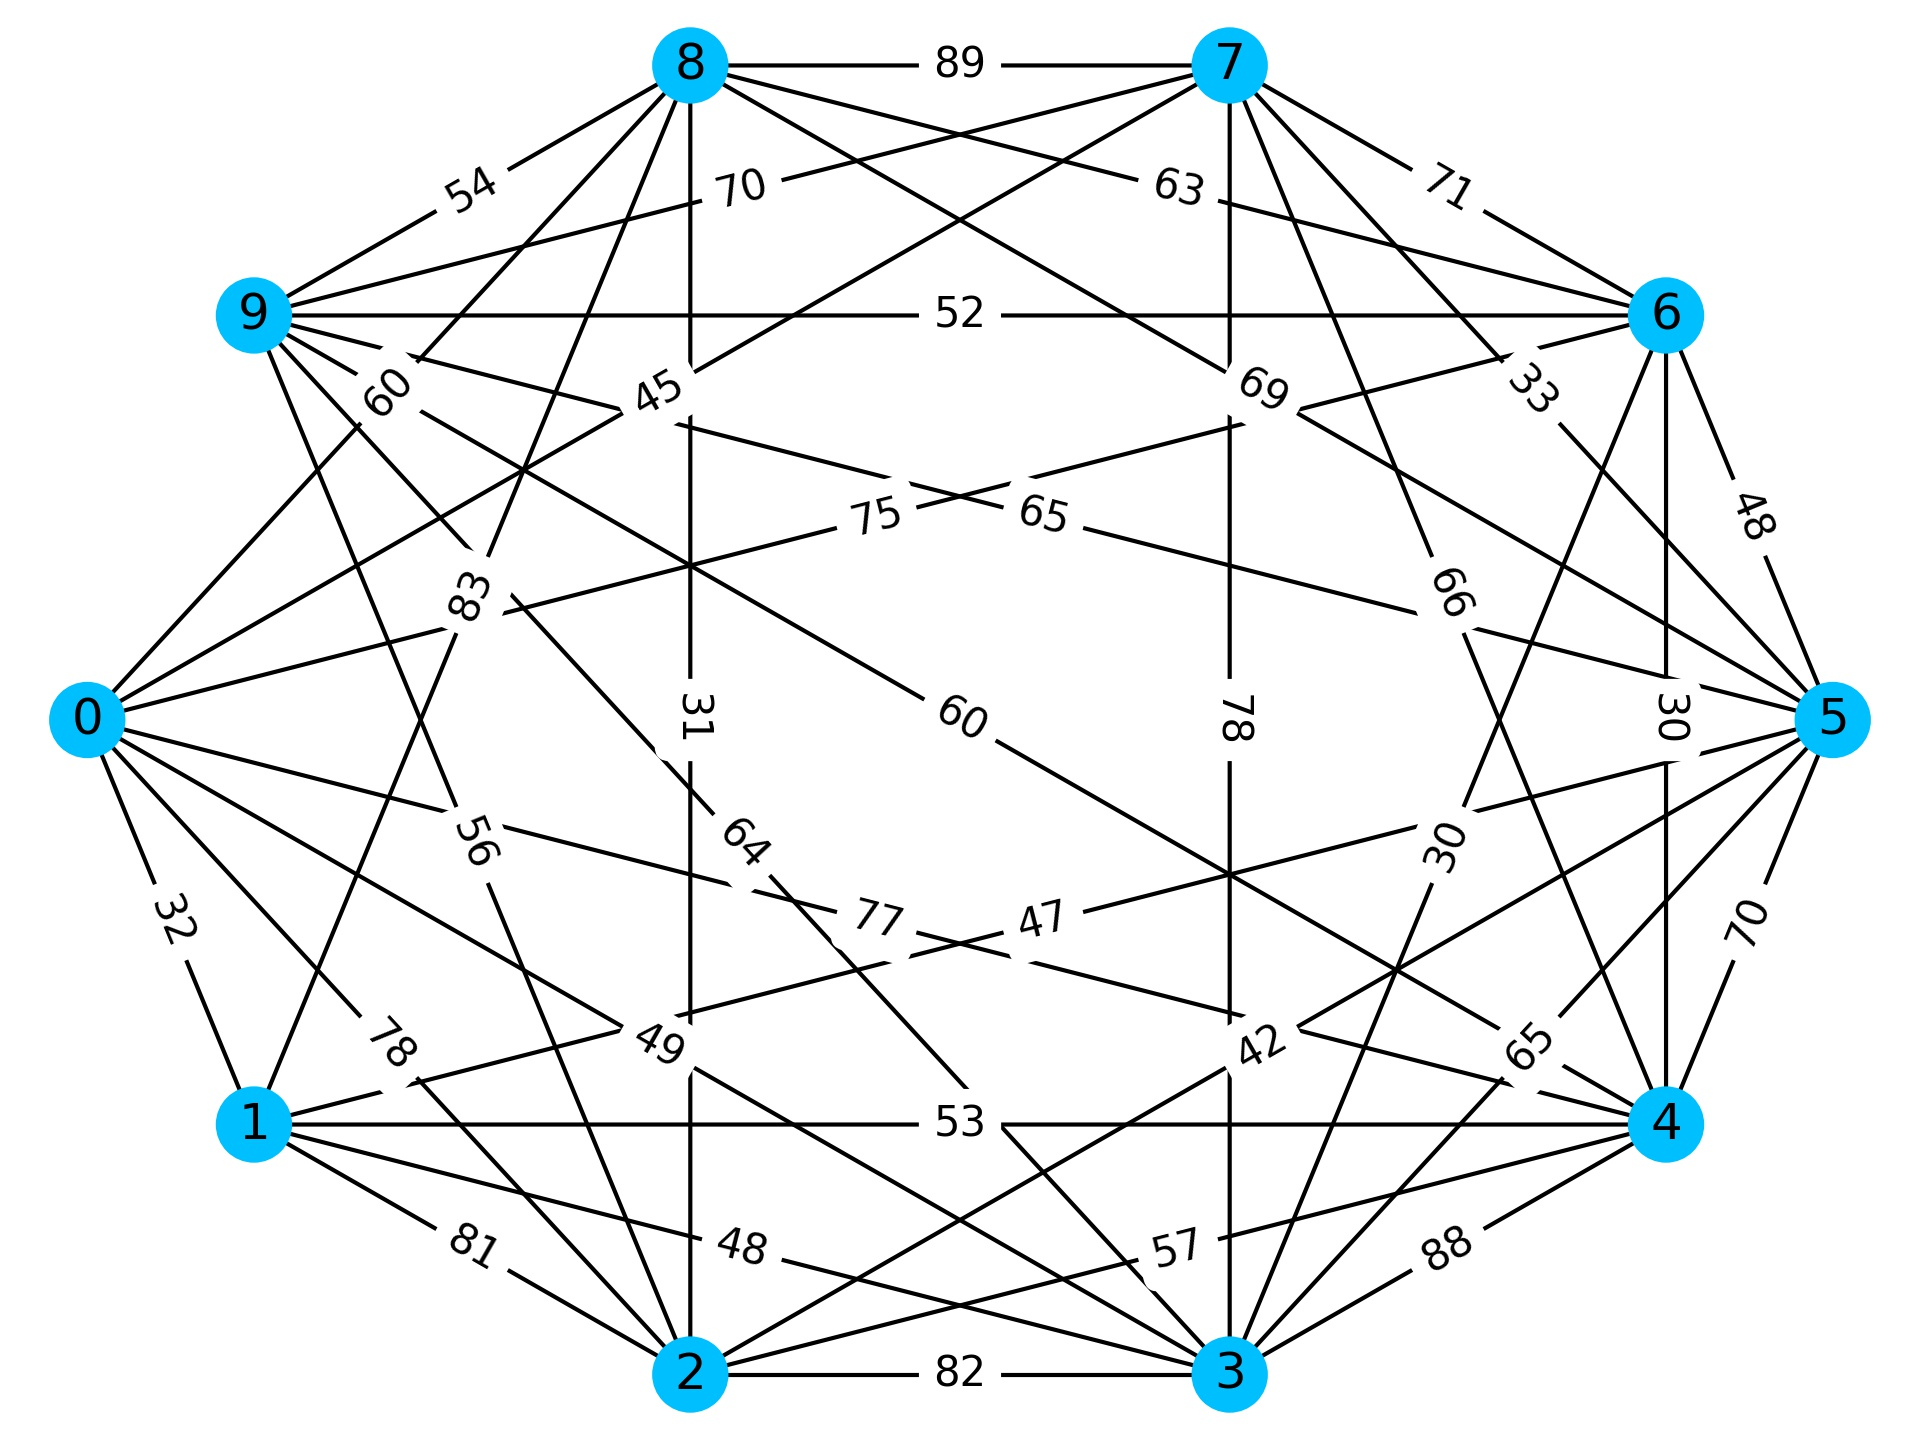
\includegraphics[width=1\linewidth]{slike/300dpi/0d.jpg}
\caption{Početni graf}
\end{figure}

Pretpostavit će se da pretraga minimalnog povezujućeg stabla počinje od čvora 0. Na narednim figurama će biti prikazani svi koraci, odnosno sve iteracije potrebne za pronalazak MST-a.
Inicijalno u skupu posjećenih čvorova $U$ se nalazi odabrani početni čvor 0 od kojeg pretraga kreće, skup grana stabla $E'$ je prazan. U while petlji se poziva metoda \texttt{pronadji\_min} i ona evaluira grane $\{0,1\}$, $\{0,2\}$, $\{0,3\}$, $\{0,4\}$, $\{0,6\}$, $\{0,7\}$ i $\{0,8\}$ tj. evaluiraju se sve grane koje nisu označene i čija je težina nije jednaka beskonačnosti. Kako je iz priloženog grafa vidljivo, najmanju težinu ima grana $\{0,1\}$ tako da se ta grana dodaje u skup $E'$, a čvor 1 u skup posjećenih čvorova $U$.


\begin{figure}[H]
\begin{center}
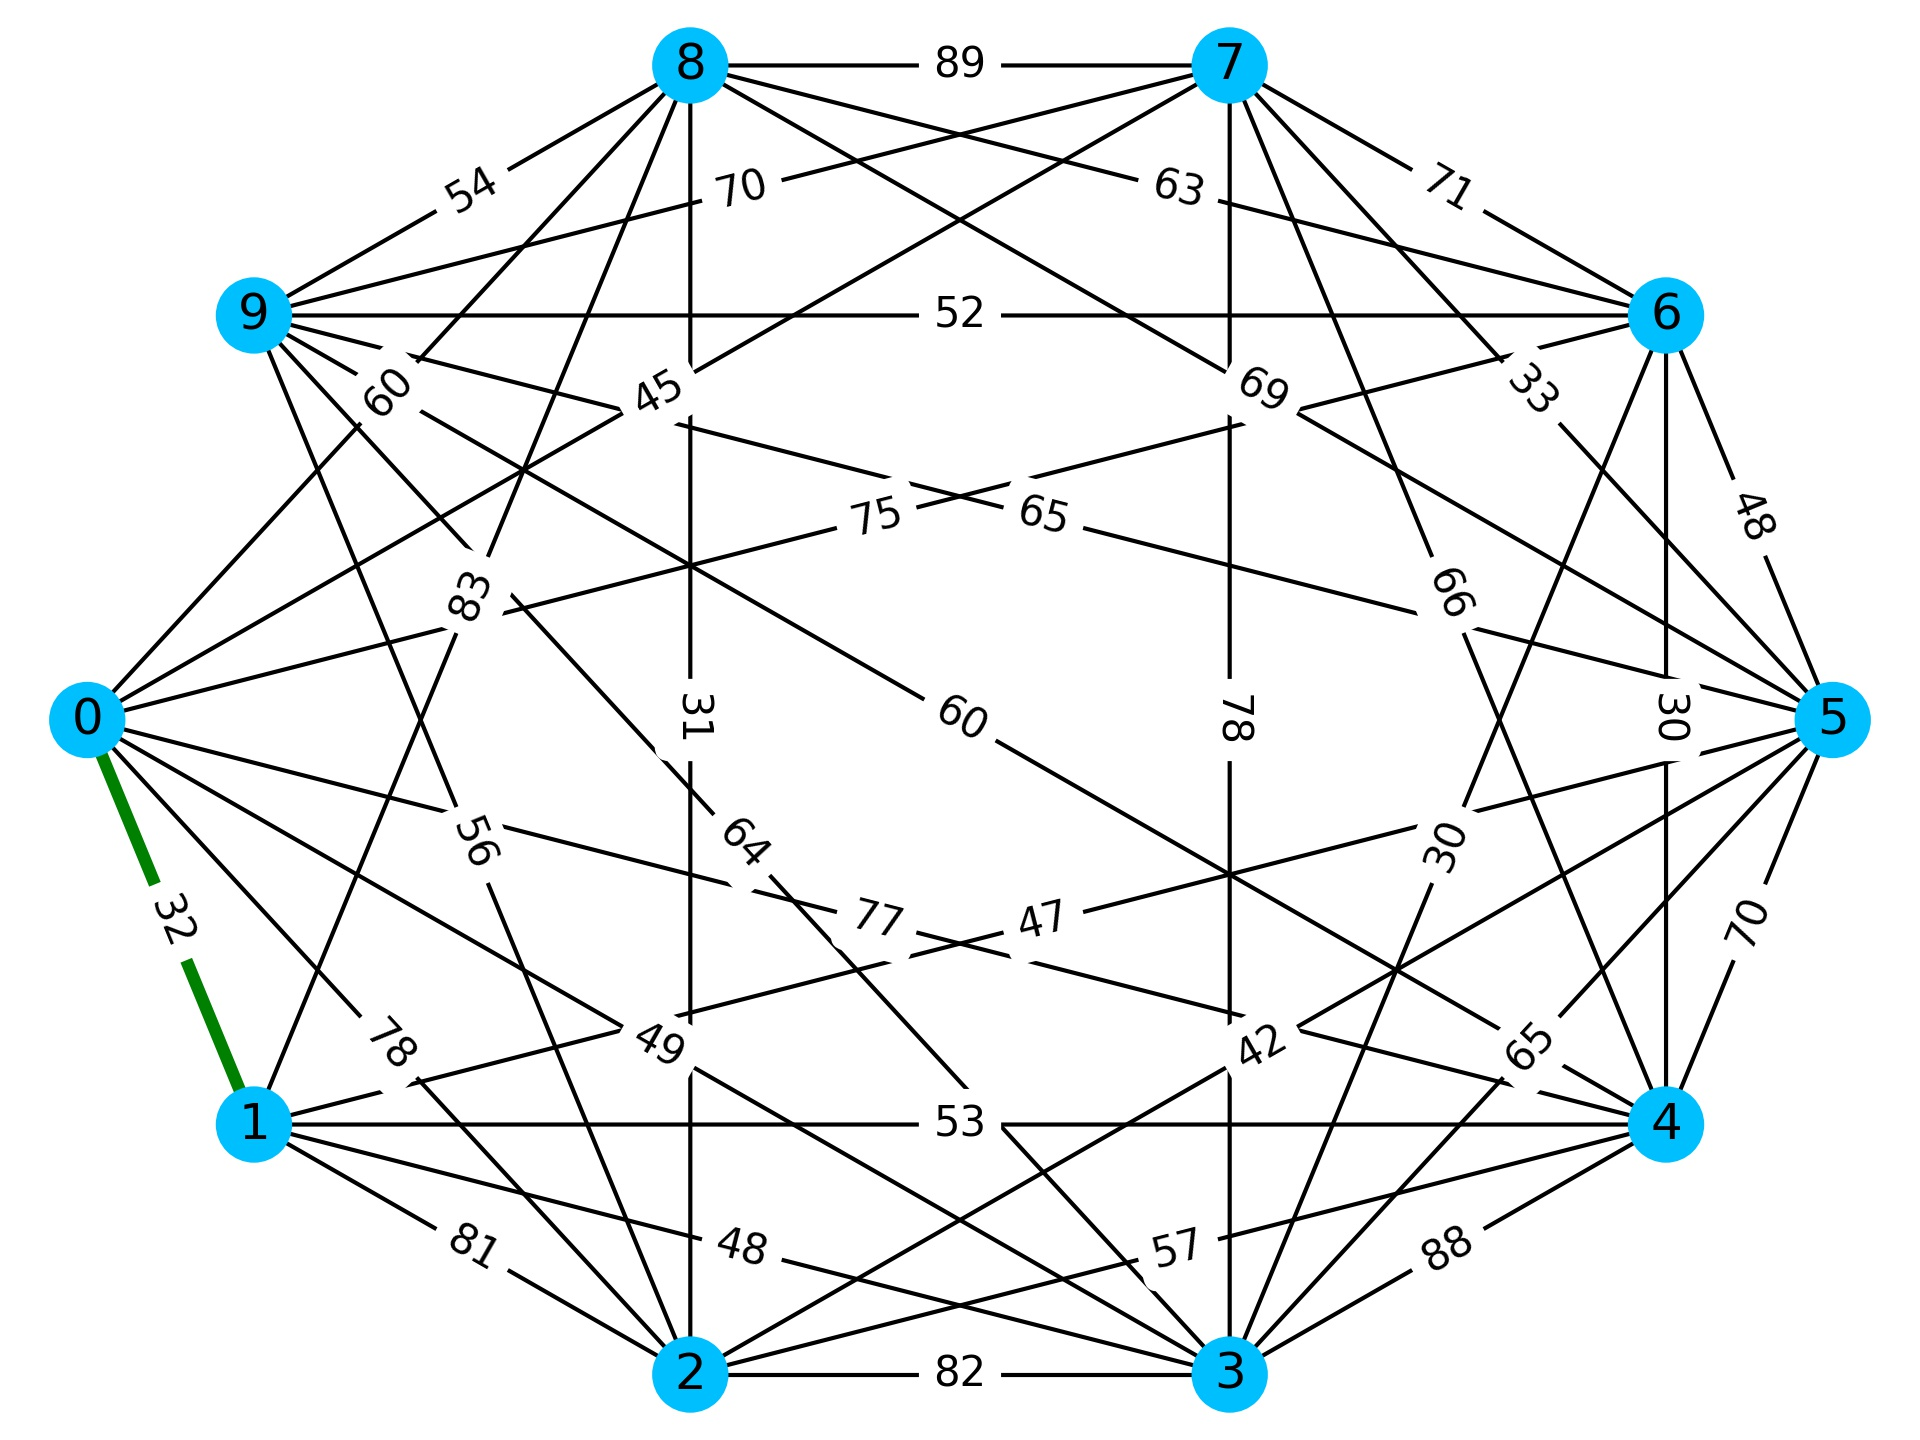
\includegraphics[width=1\linewidth]{slike/300dpi/1d.jpg}
\caption{Prva iteracija}
\label{figmat}
\end{center}

Nakon prvog koraka u skupu posjećenih čvorova se nalaze čvorovi 0 i 1, što znači da će vrijediti $V-U = \{2,3,4,5,6,7,8,9\}$. Na osnovu izraza iz pseudokoda \ref{algo} (5 linija), algoritam će razmatrati sljedeći skup grana: $\{0,2\}$, $\{0,3\}$, $\{0,4\}$, $\{0,6\}$, $\{0,7\}$, $\{0,8\}$, $\{1,2\}$, $\{1,3\}$, $\{1,4\}$, $\{1,6\}$, $\{1,7\}$ i $\{1,8\}$. U navedenom skupu grana $\{0,7\}$ ima najmanju težinu 45. Ova grana se također uvodi u skup $E'$, a čvor 7 u skup posjećenih čvorova. Kako ostatak algoritma teče na potpuno isti način, bez dodatnih objašnjenja će biti prikazan ostatak koraka (iteracija algoritma). U svakoj iteraciji je zelenom bojom označena grana koja je u toj iteraciji odabrana dok grane podebljane crnom bojom predstavljaju trenutne grane minimalno povezujućeg stabla.

\begin{figure}[H]
\centering
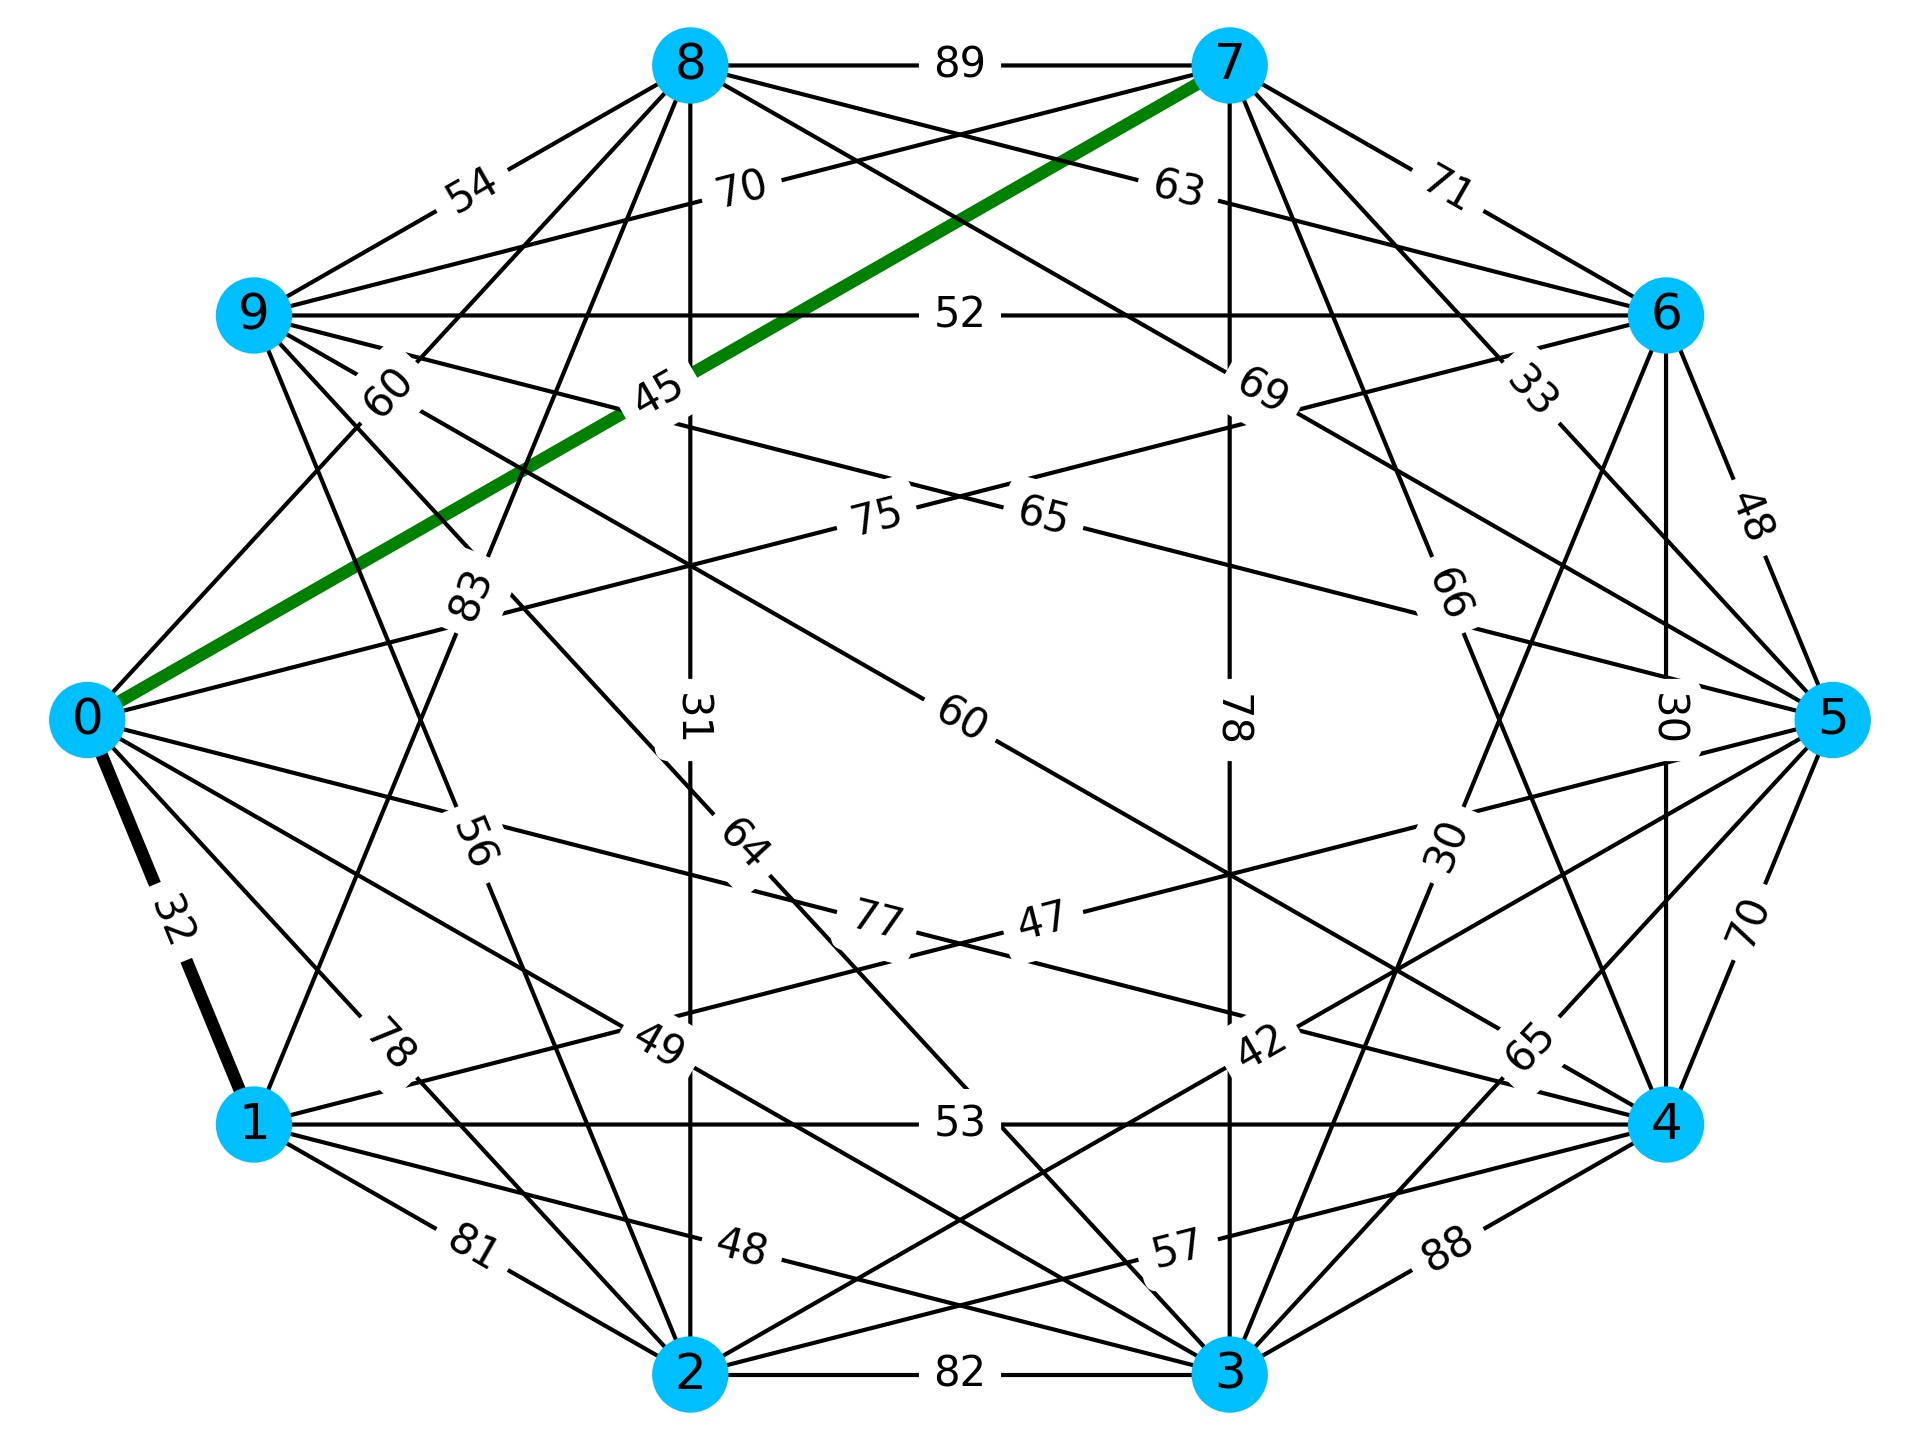
\includegraphics[width=1\linewidth]{slike/300dpi/2d.jpg}
\caption{Druga iteracija}
\label{figmat}
\end{figure}

\end{figure}



\begin{figure}[H]
\centering
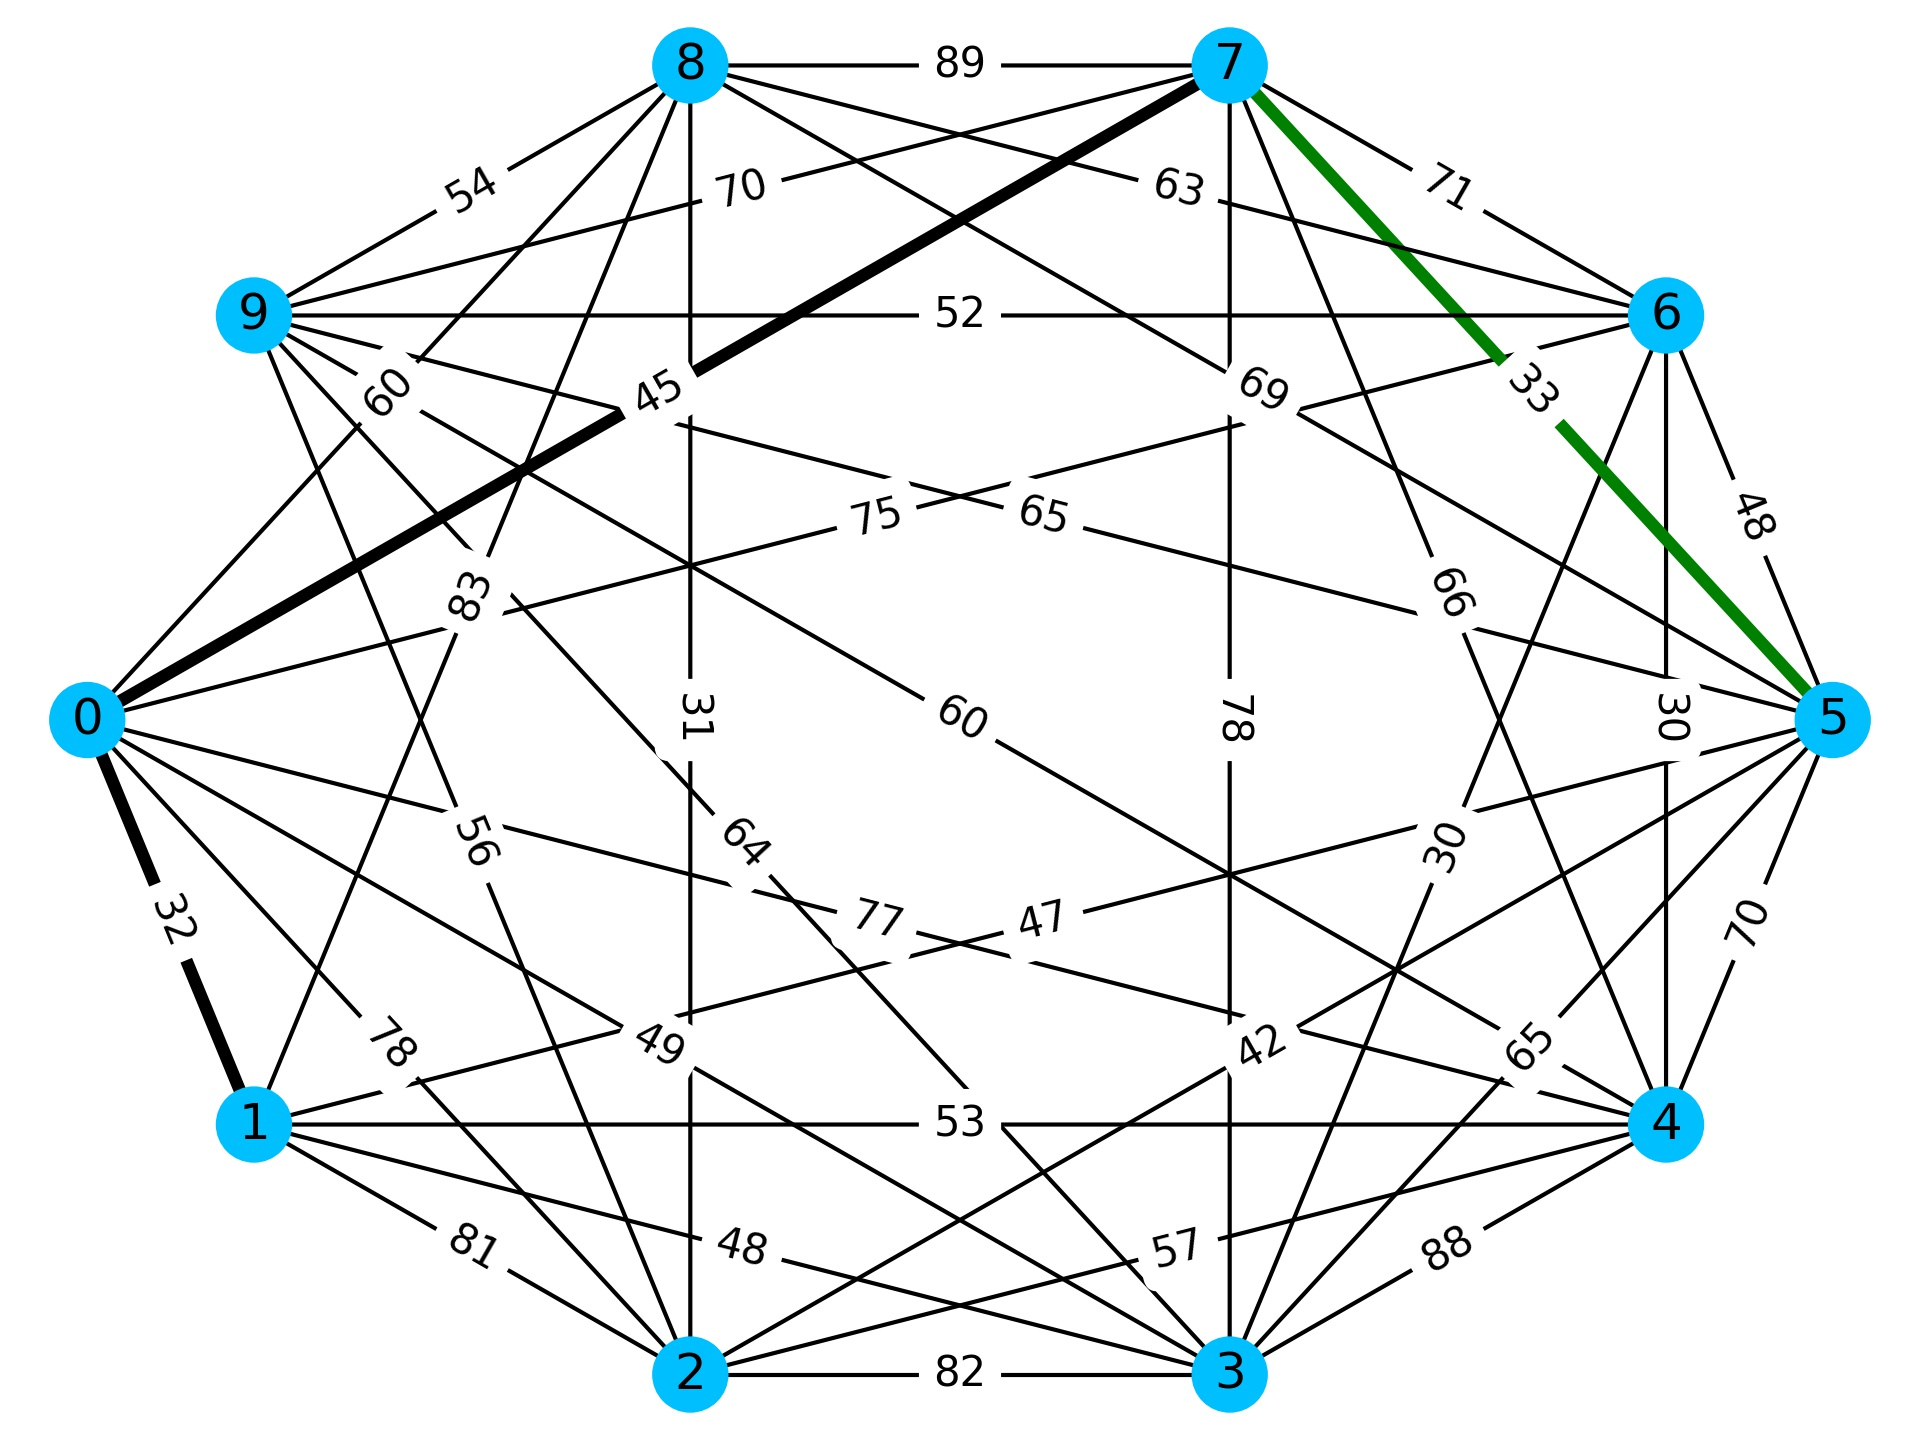
\includegraphics[width=1\linewidth]{slike/300dpi/3d.jpg}
\caption{Treća iteracija}
\label{figmat}
\end{figure}

\begin{figure}[H]
\centering
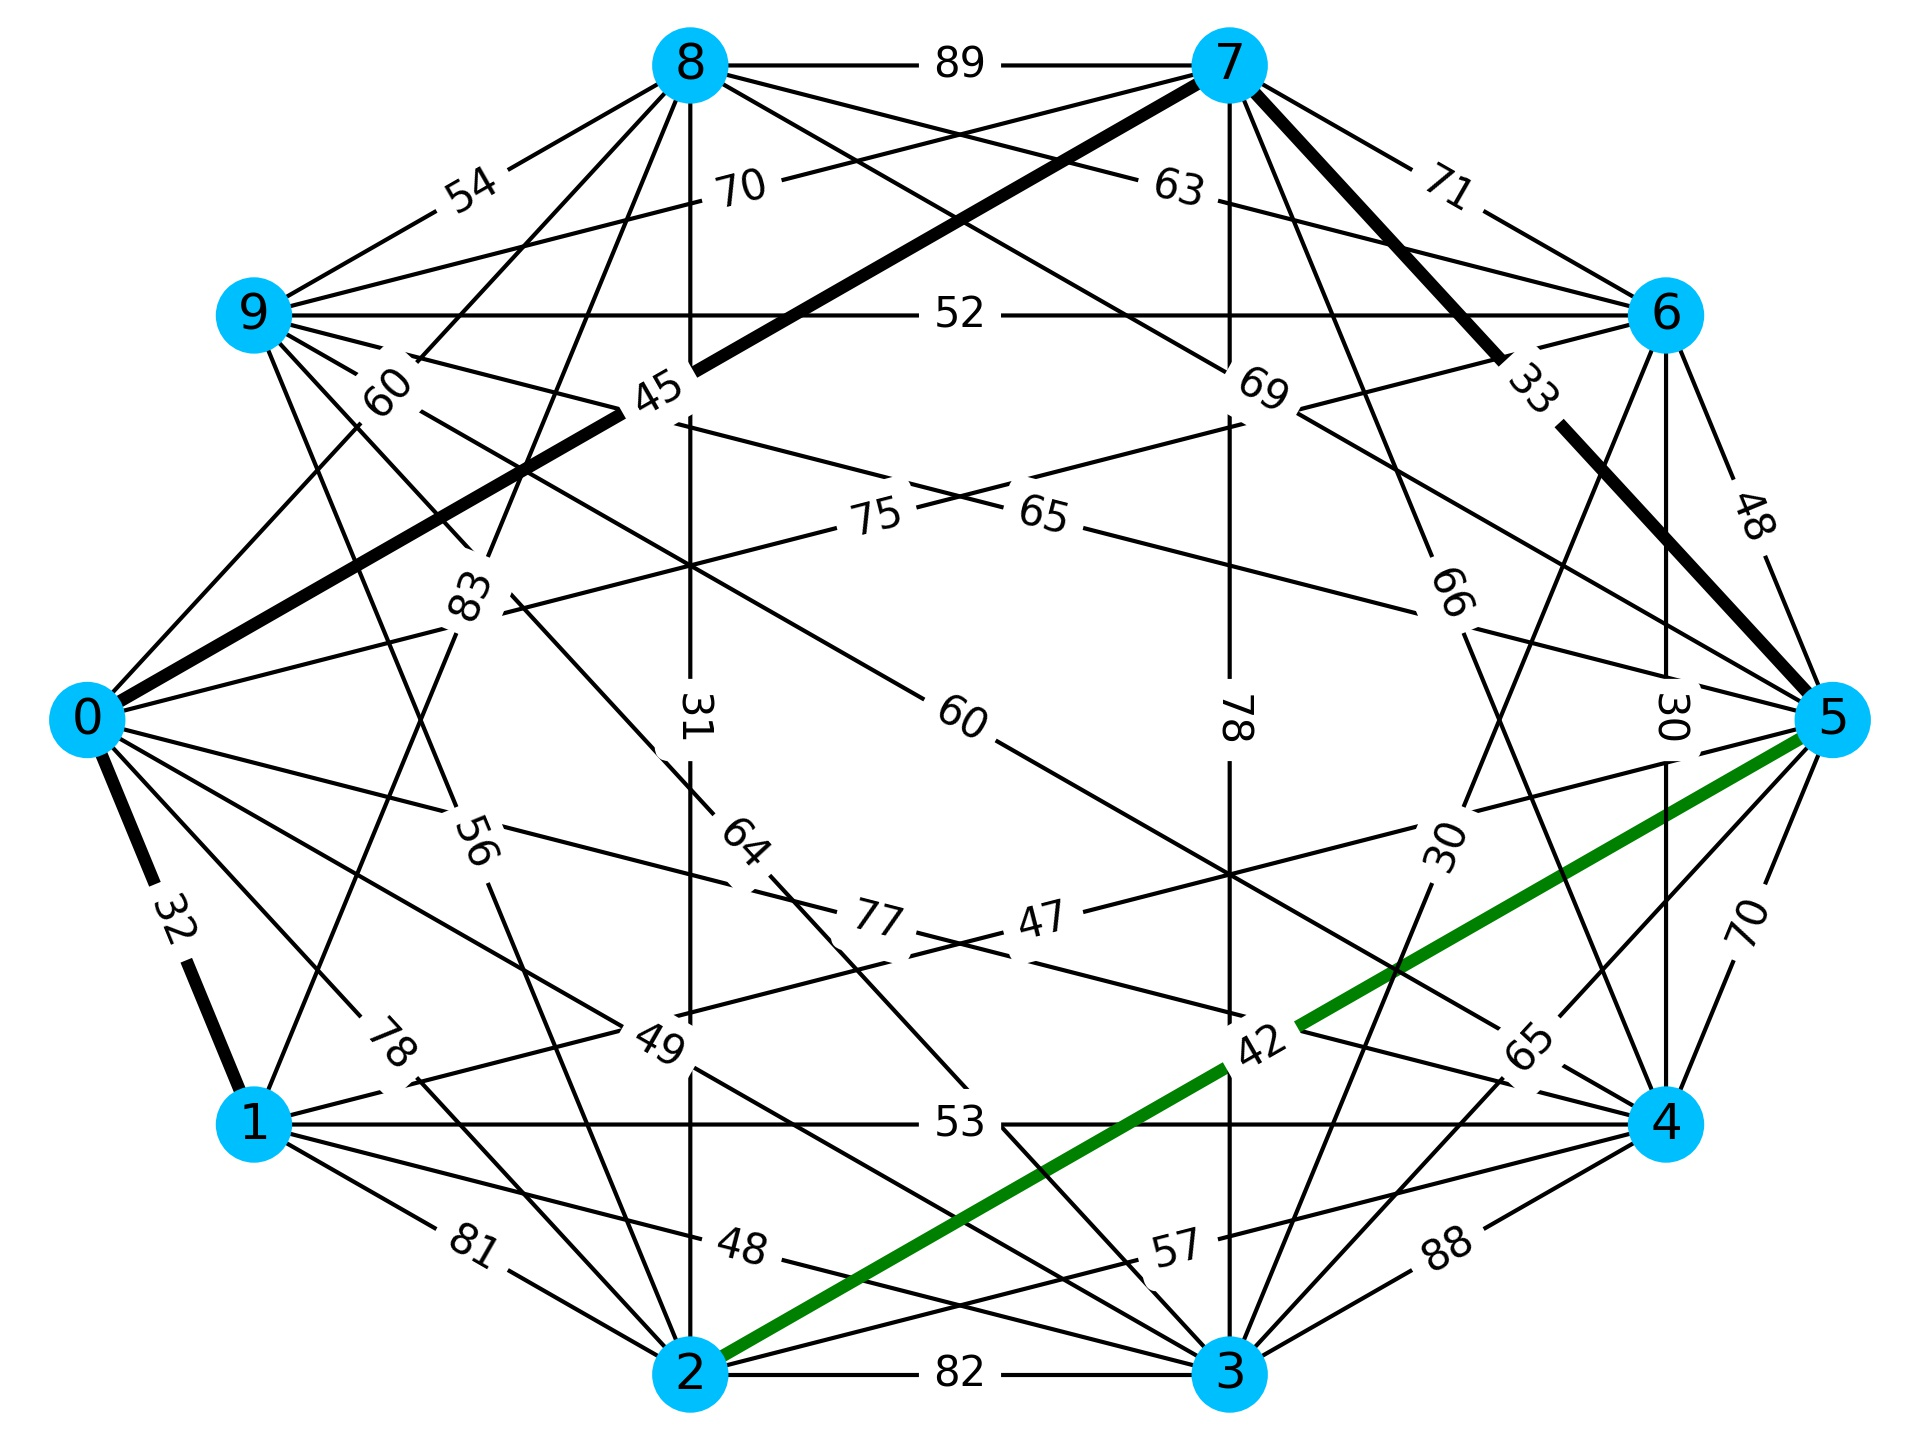
\includegraphics[width=1\linewidth]{slike/300dpi/4d.jpg}
\caption{Četvrta iteracija}
\label{figmat}
\end{figure}

\begin{figure}[H]
\centering
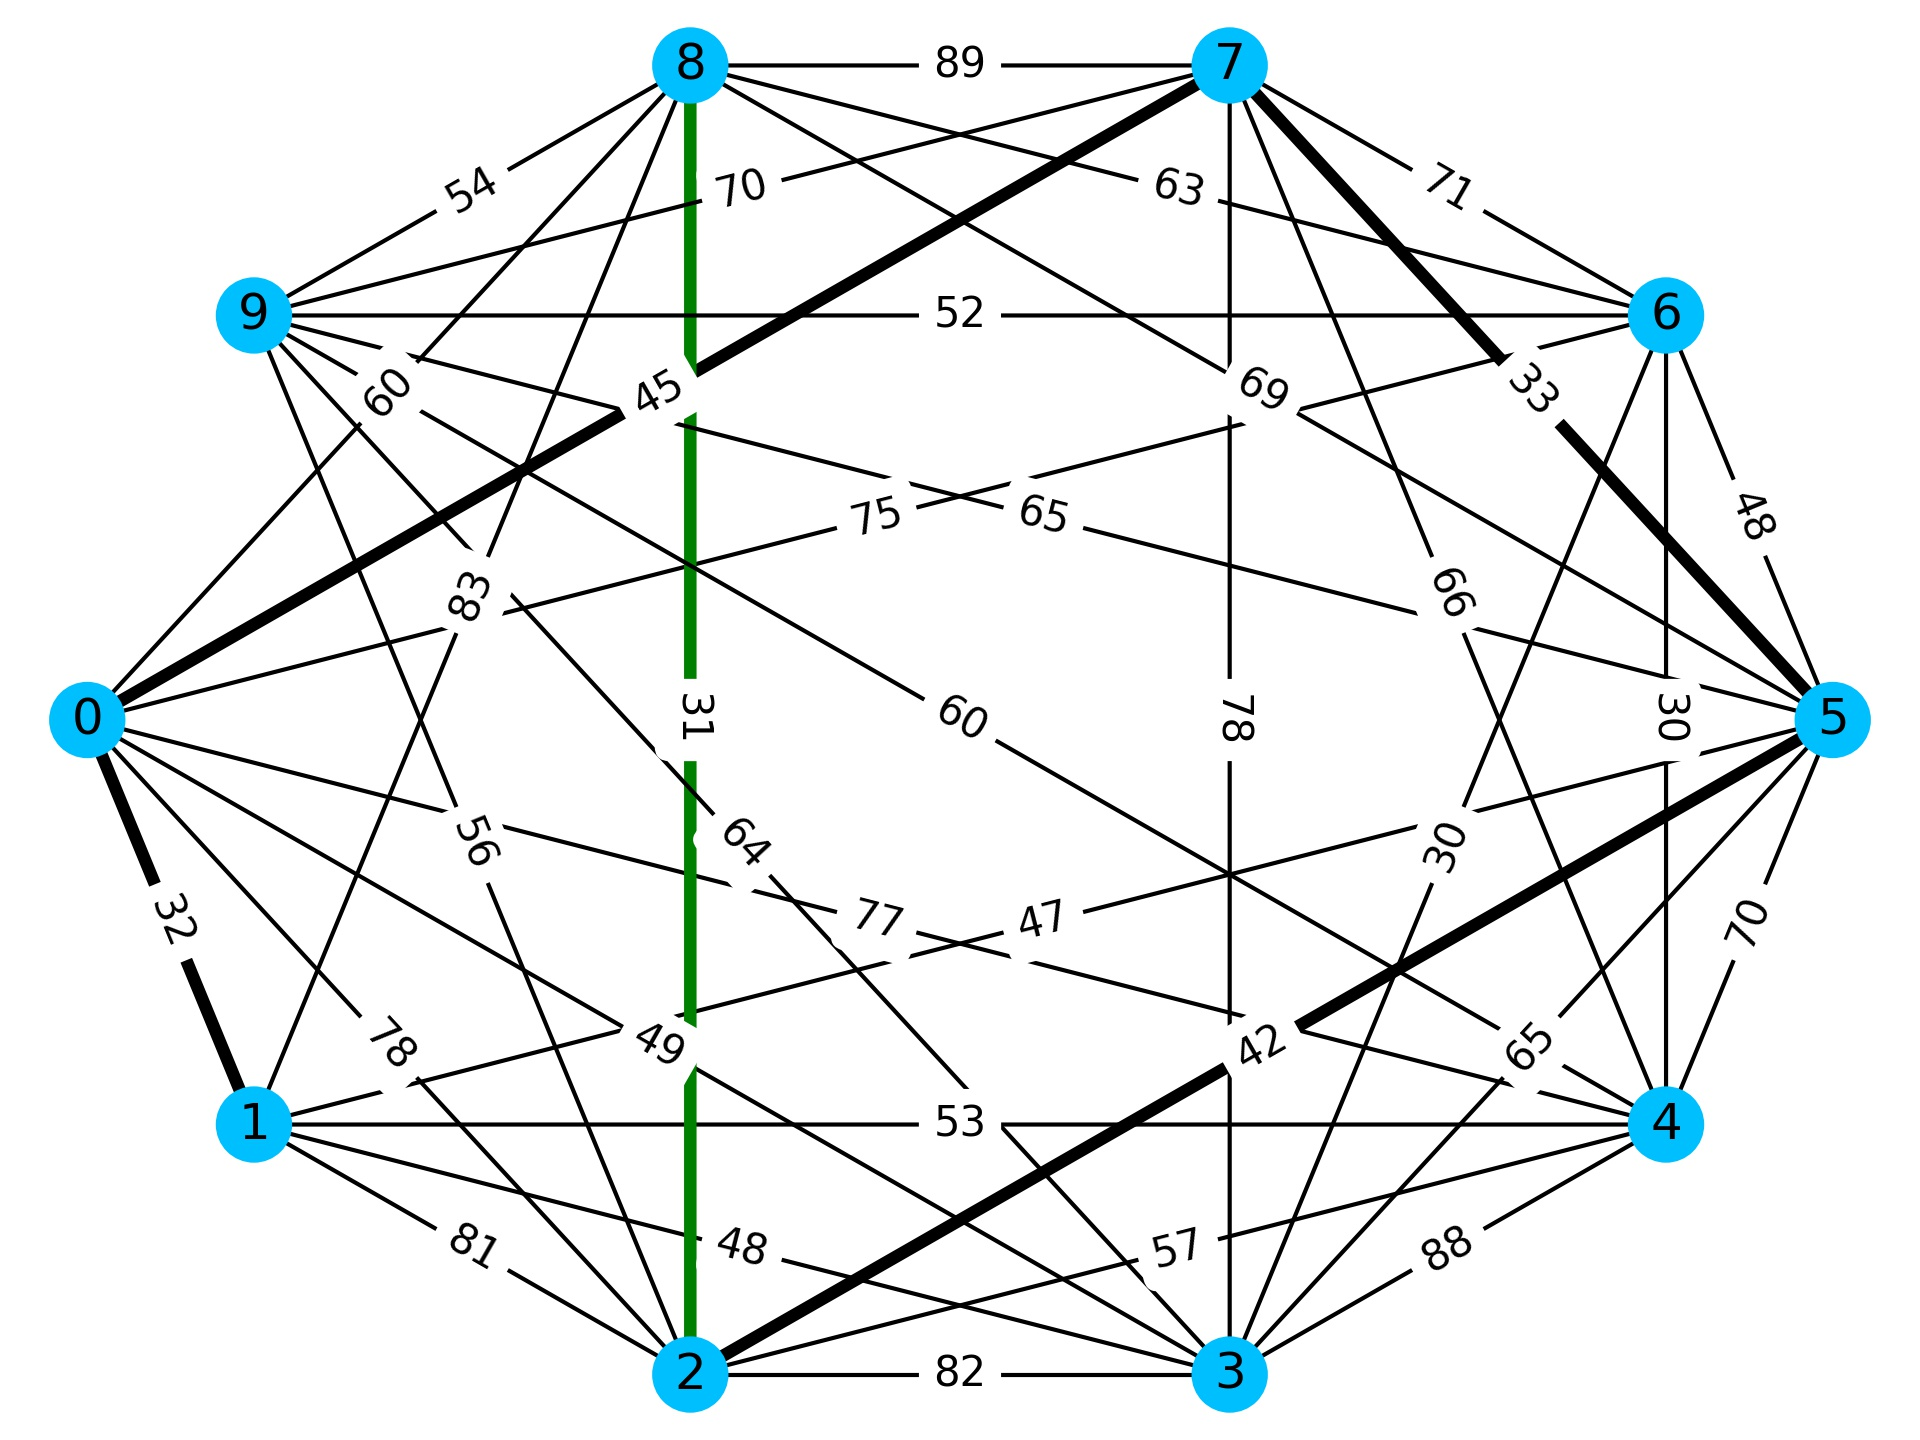
\includegraphics[width=1\linewidth]{slike/300dpi/5d.jpg}
\caption{Peta iteracija}
\label{figmat}
\end{figure}

\begin{figure}[H]
\centering
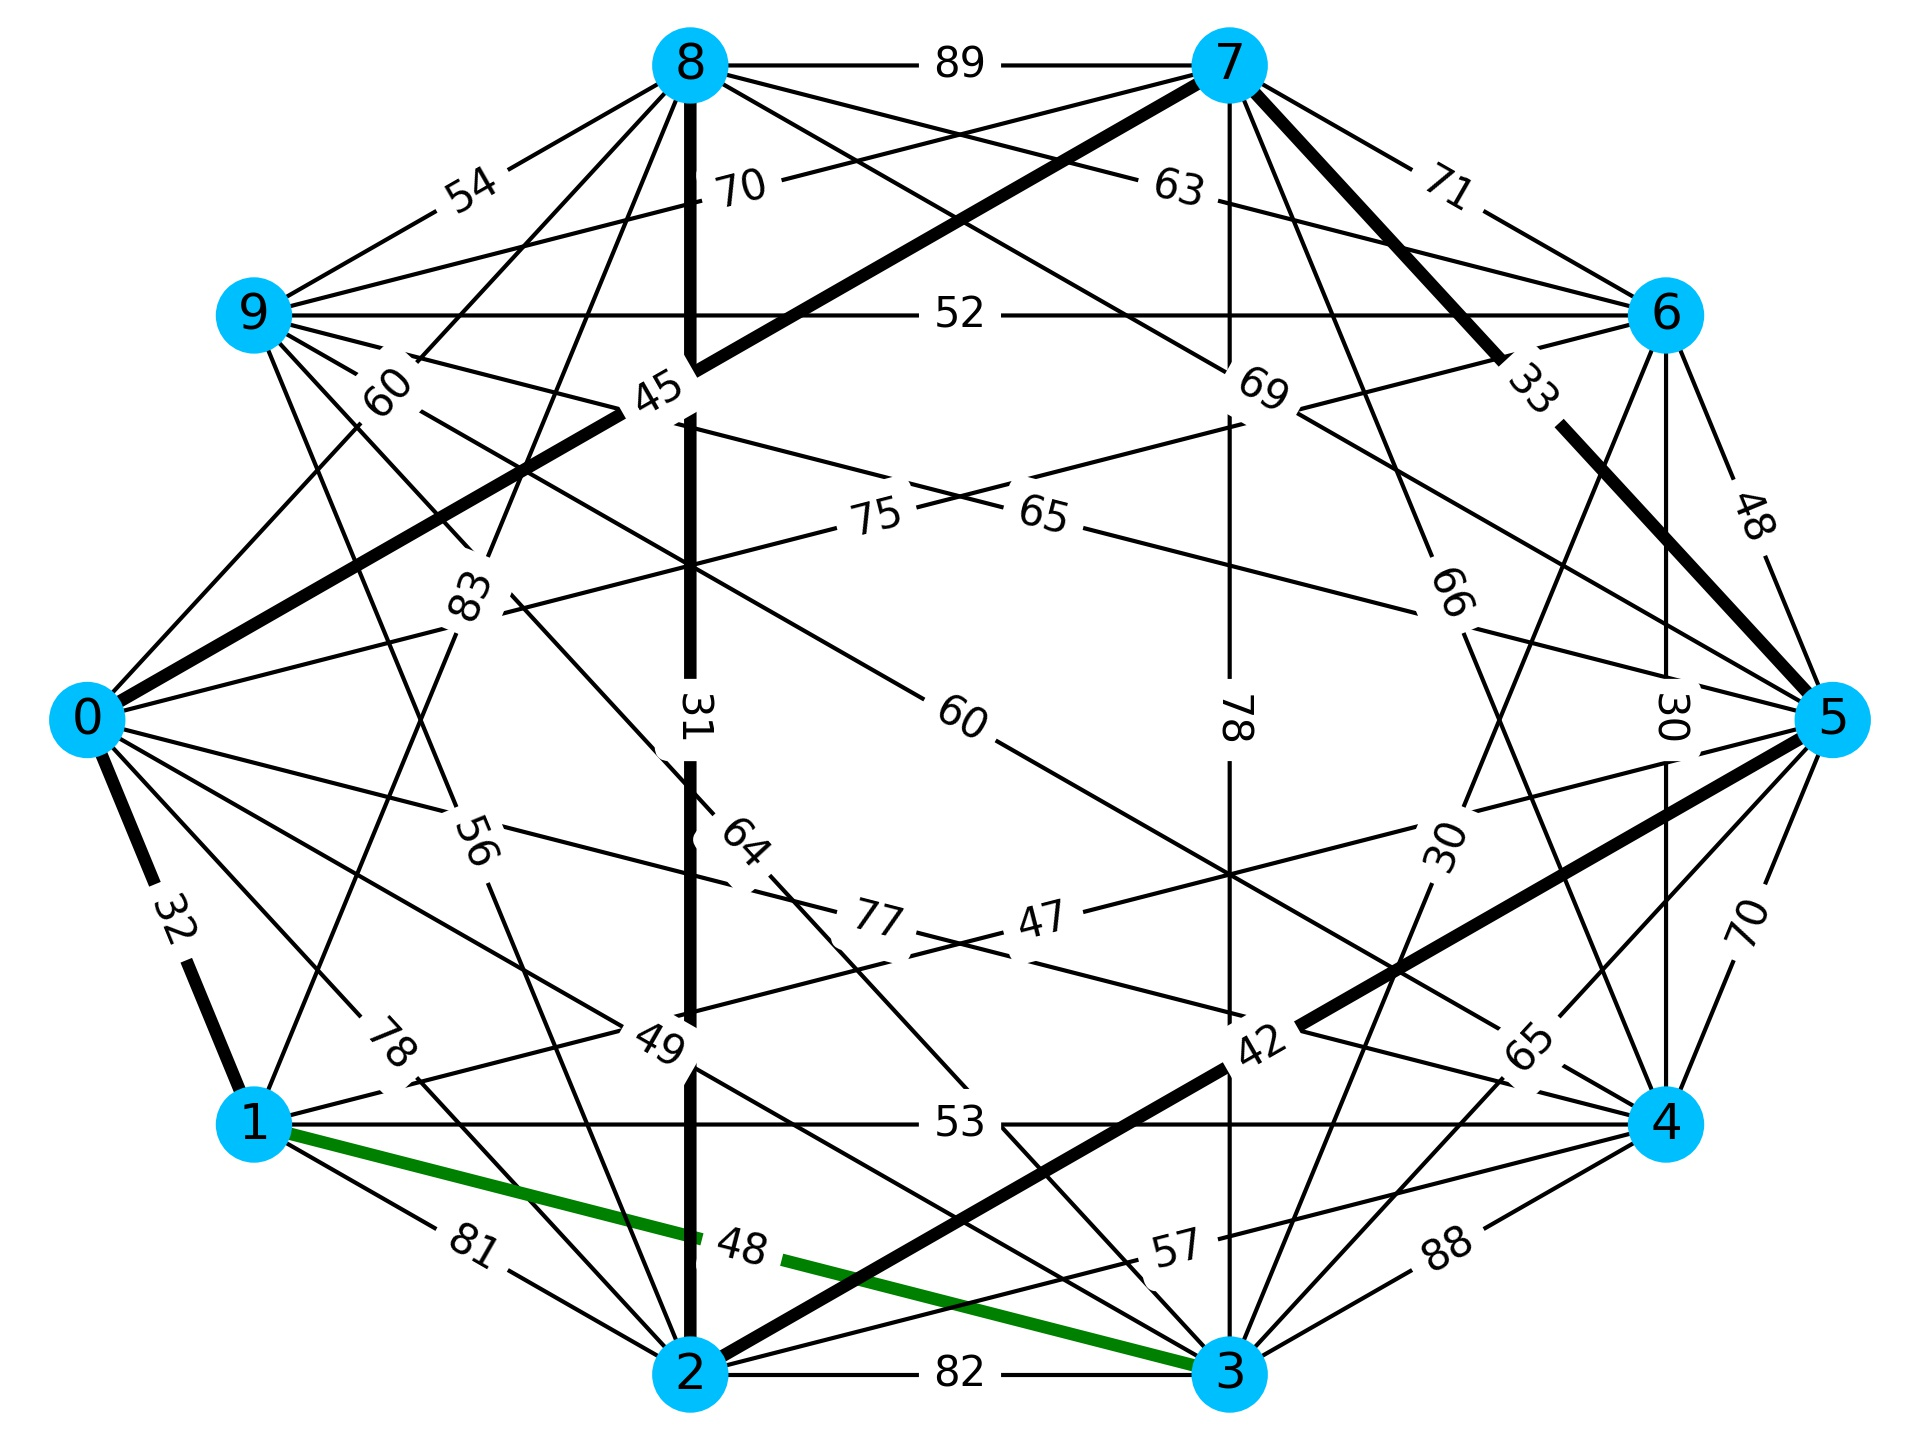
\includegraphics[width=1\linewidth]{slike/300dpi/6d.jpg}
\caption{Šesta iteracija}
\label{figmat}
\end{figure}

\begin{figure}[H]
\centering
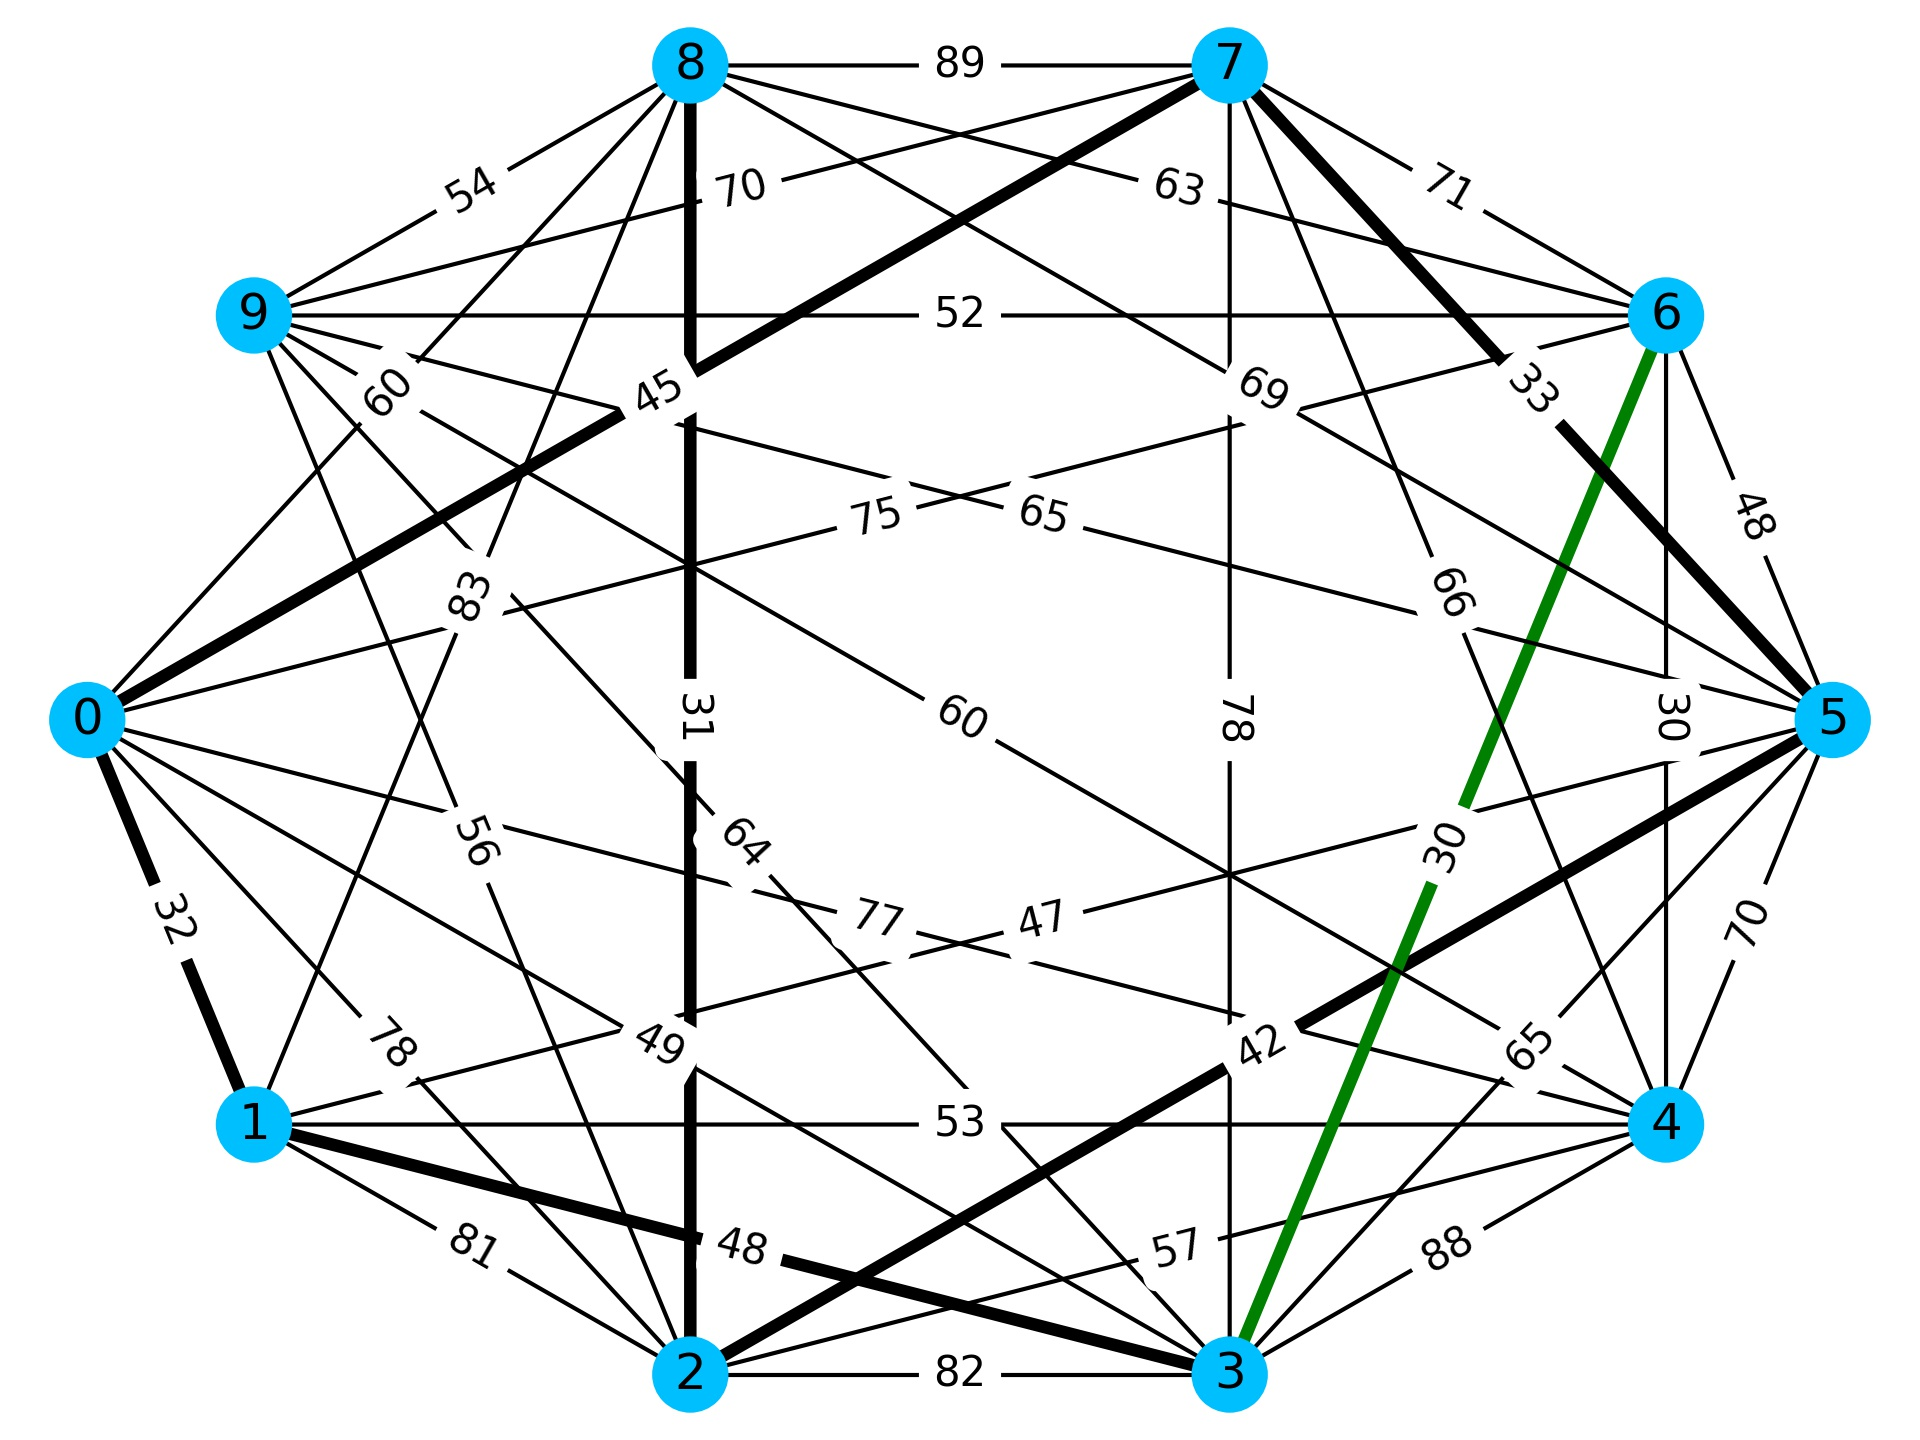
\includegraphics[width=1\linewidth]{slike/300dpi/7d.jpg}
\caption{Sedma iteracija}
\label{figmat}
\end{figure}

\begin{figure}[H]
\centering
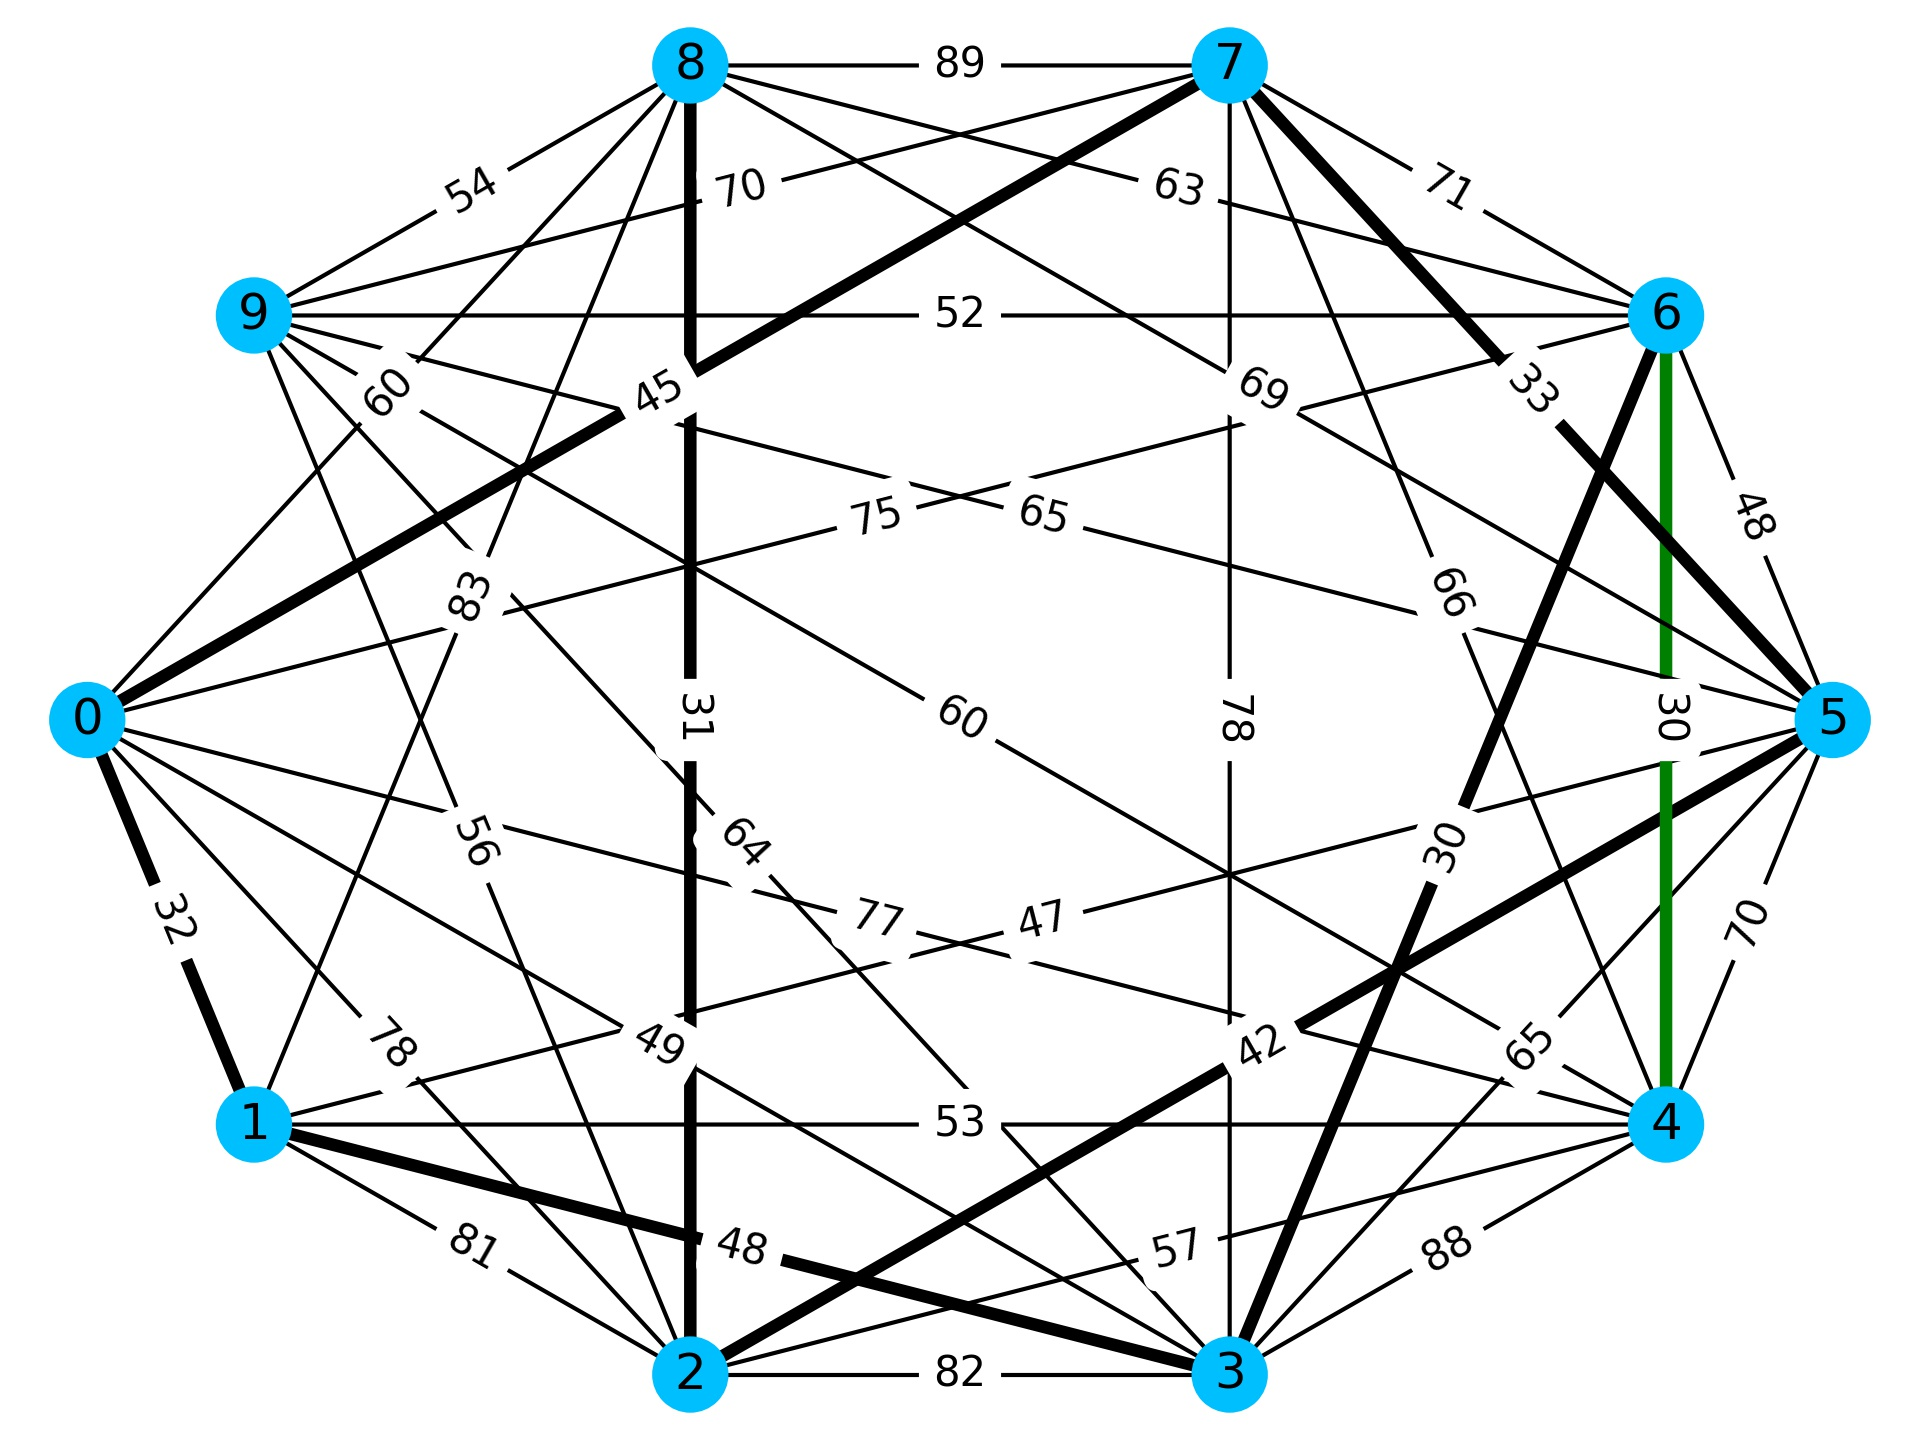
\includegraphics[width=1\linewidth]{slike/300dpi/8d.jpg}
\caption{Osma iteracija}
\label{figmat}
\end{figure}

\begin{figure}[H]
\centering
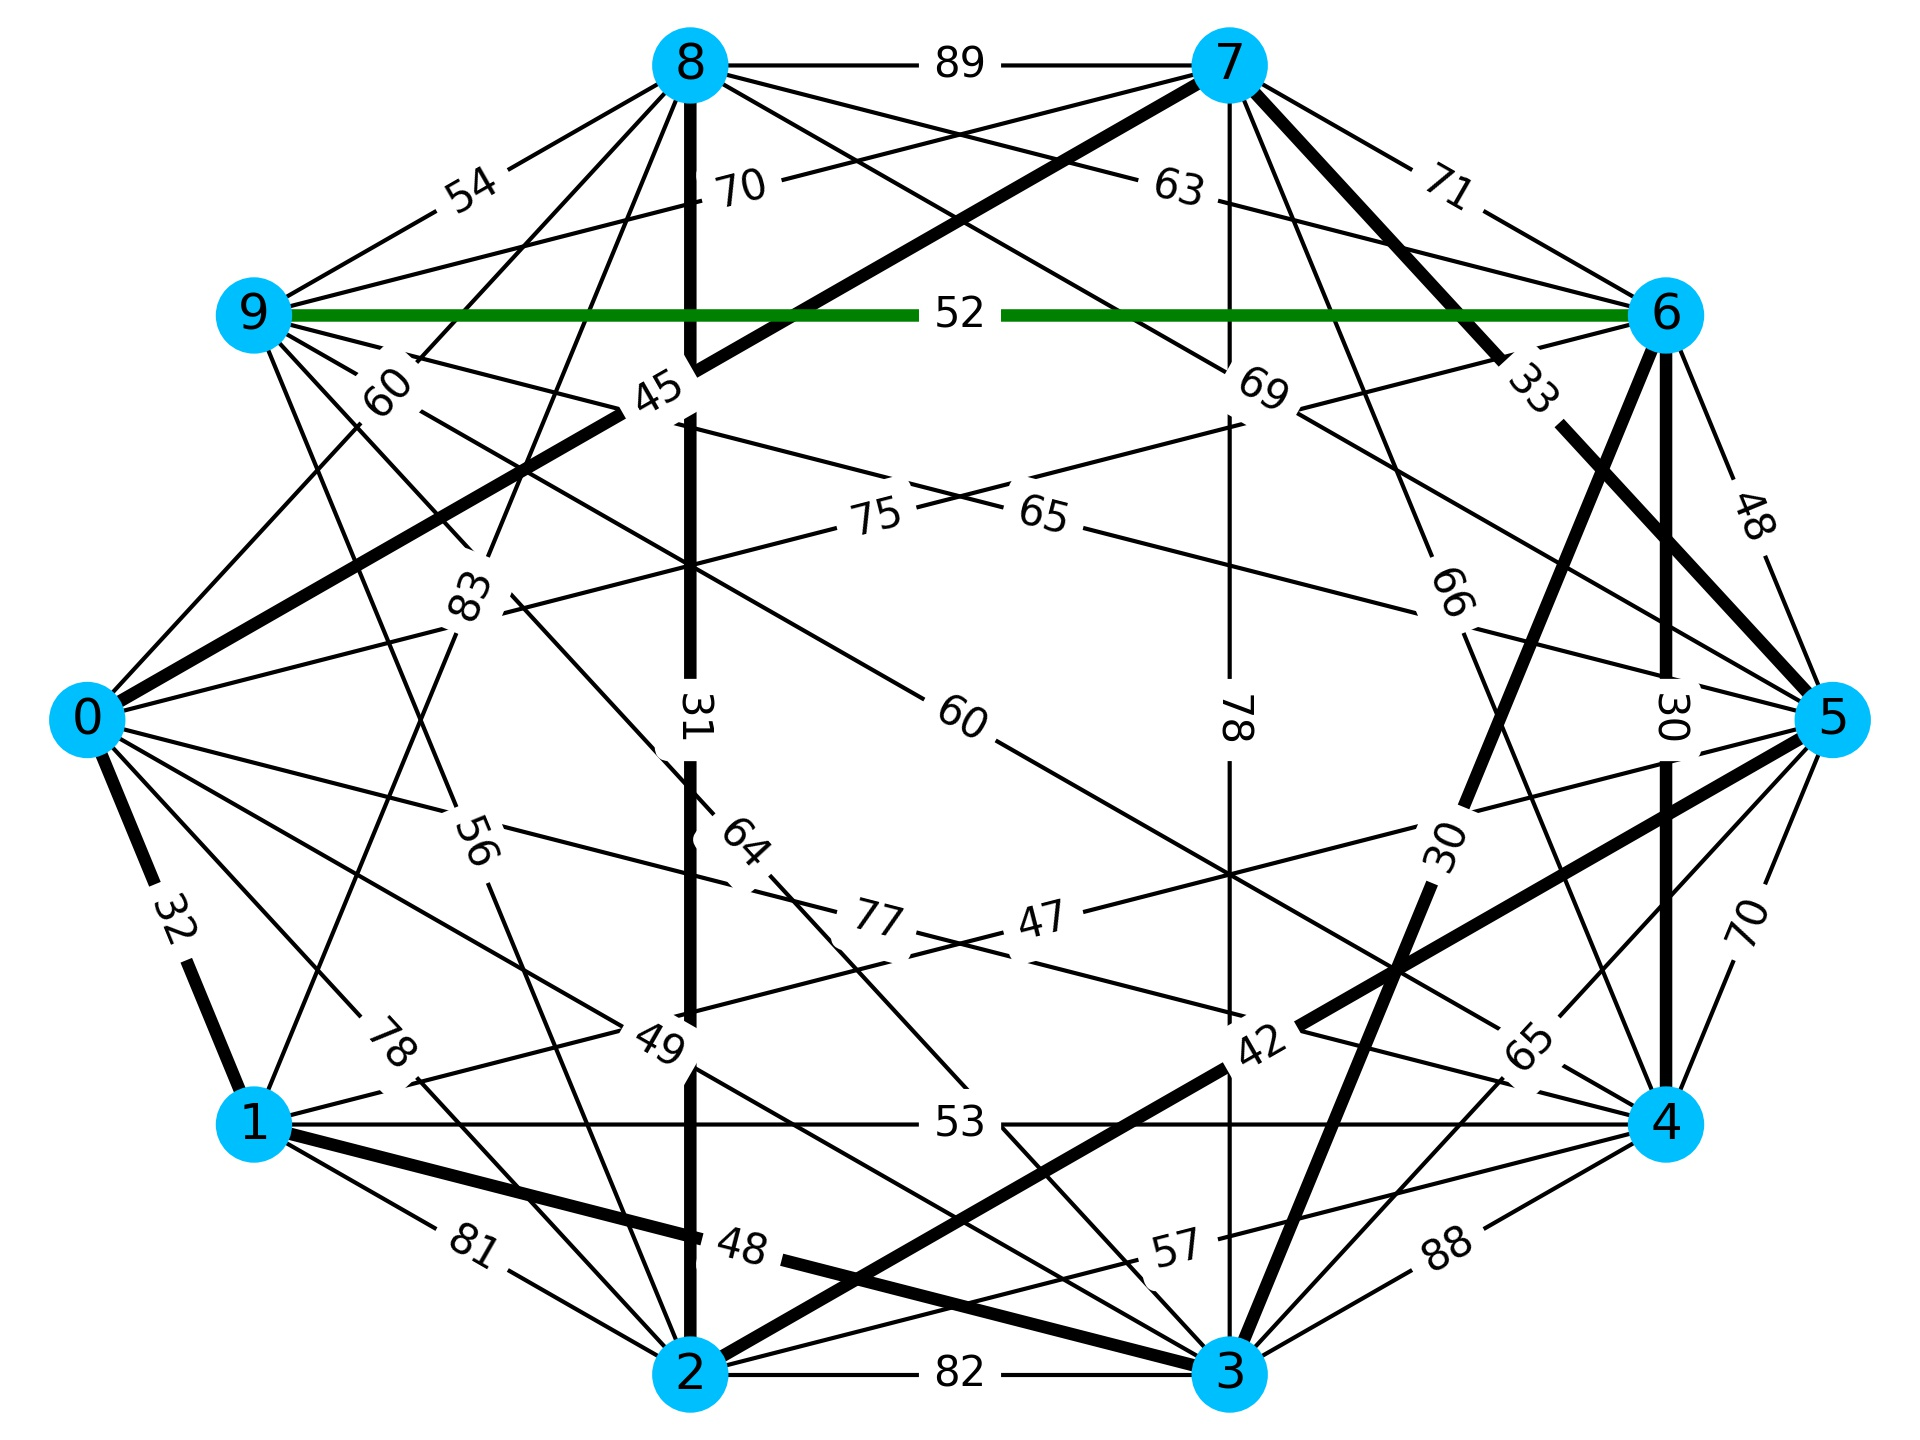
\includegraphics[width=1\linewidth]{slike/300dpi/9d.jpg}
\caption{Deveta iteracija}
\label{figmat}
\end{figure}

\begin{figure}[H]
\centering
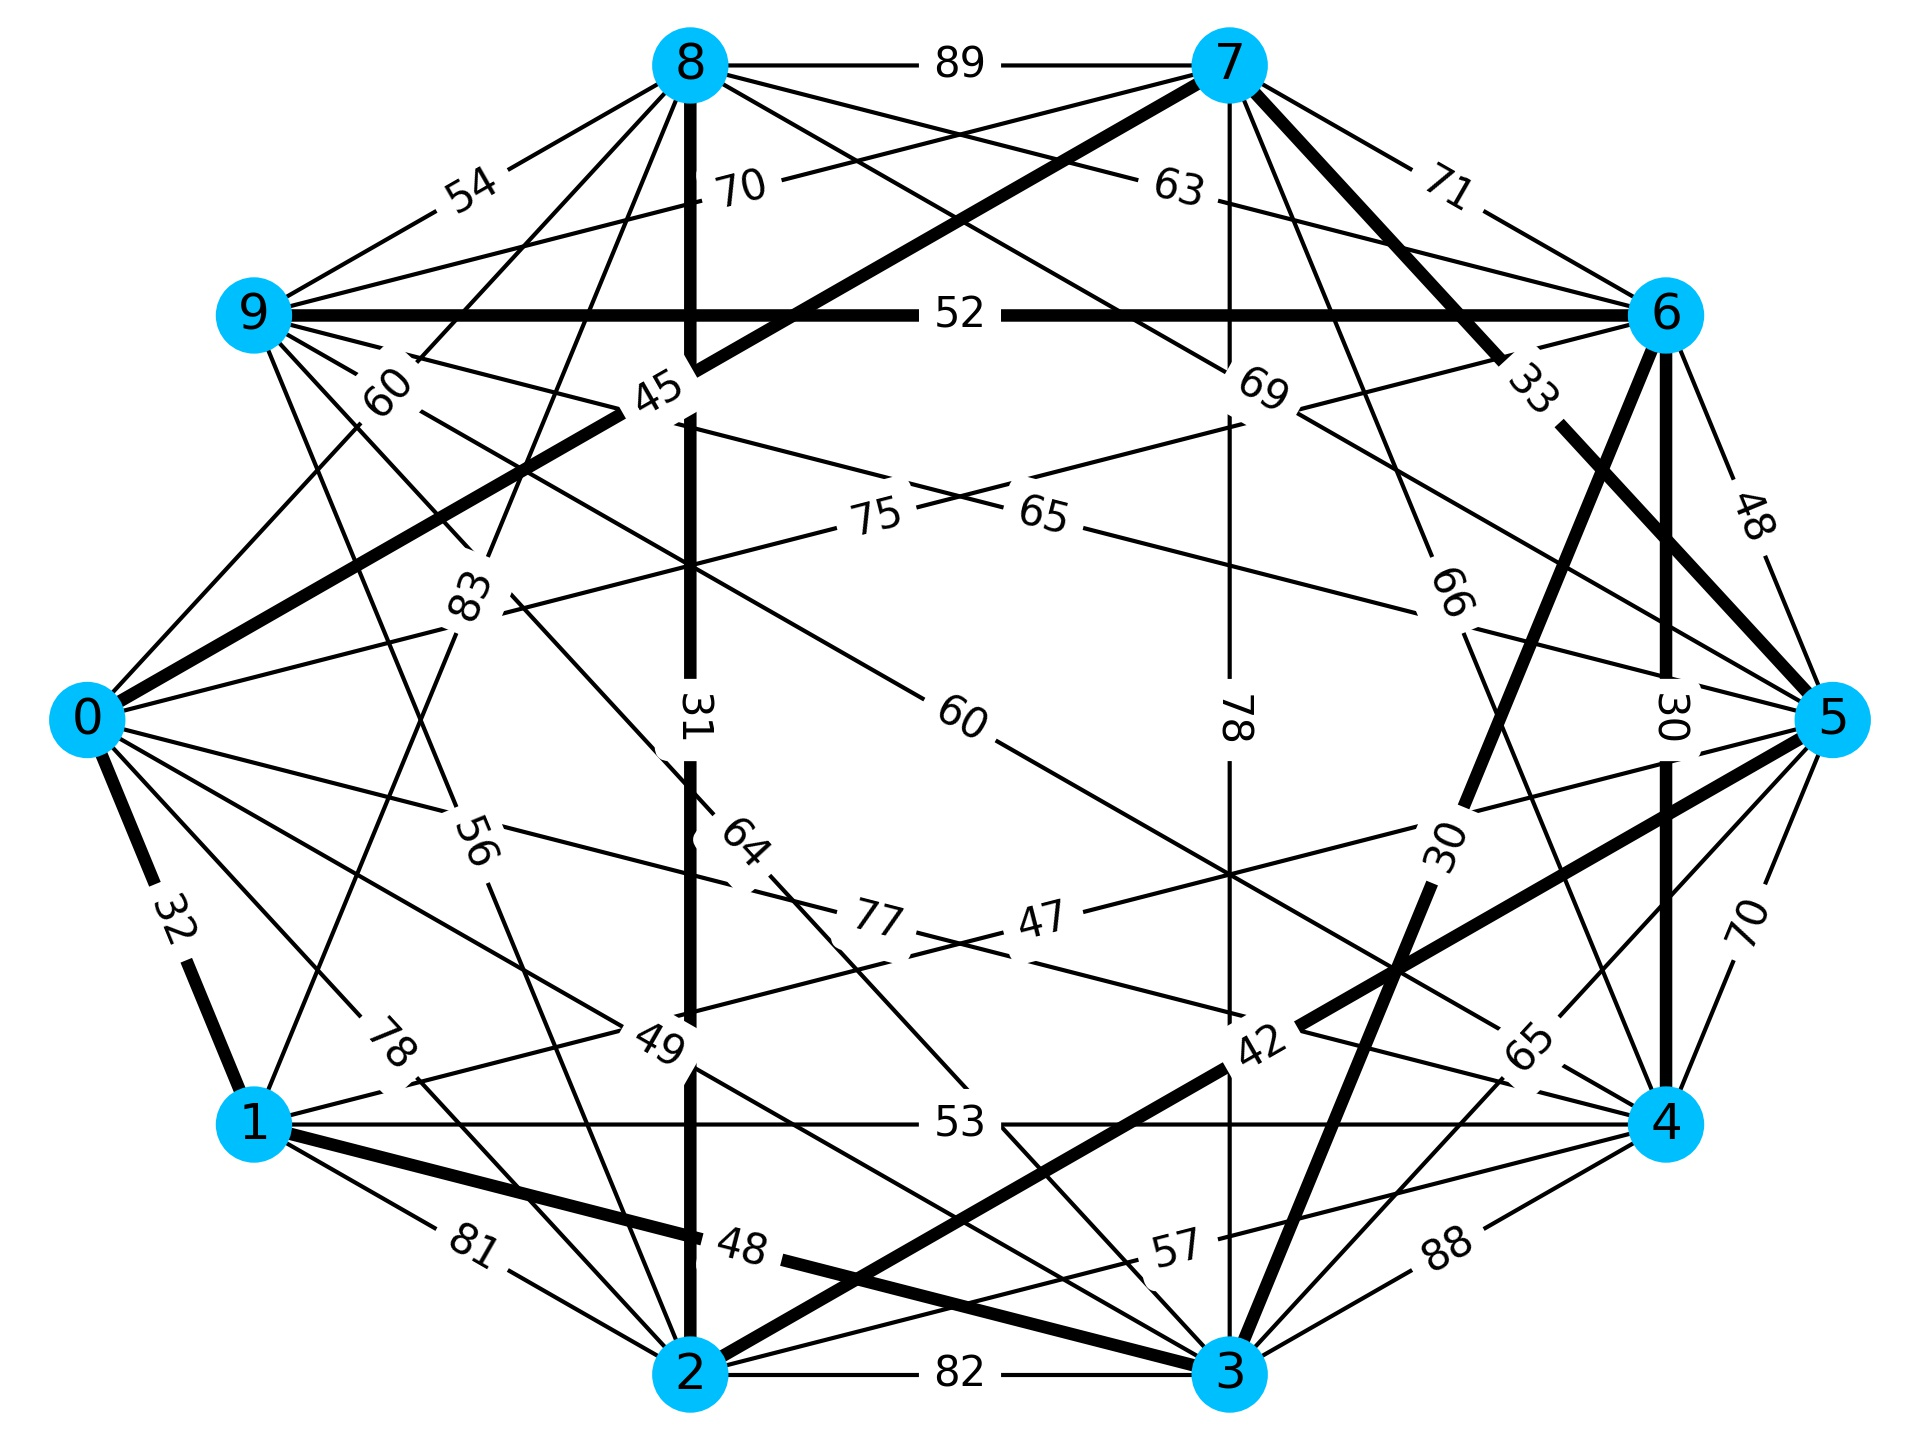
\includegraphics[width=1\linewidth]{slike/300dpi/10d.jpg}
\caption{Konačno minimalno povezujuće stablo za problem povezivanja dalekovoda}
\label{figmat}
\end{figure}

Kako početni graf sadrži 10 čvorova, kostur je formiran nakon što je izabrano 9 grana: (0,1), (0,7), (7,5), (5,2), (2,8), (1,3), (6,3), (6,4) i (6,9). Traženo minimalno povezujuće stablo ima ukupnu težinu: 32 + 45 + 33 + 42 + 31 + 48 + 30 + 30 + 52 = 343. Ono što je preostaje da se izračuna maksimalna vrijednost ušteda resursa. Da bi se to postiglo modificirat će se algoritam tako da u svakoj iteraciji uzima grane s najvećom težinom.

Odabrane grane su: (4, 5), (2, 1), (0, 6), (1, 8), (2, 3), (8, 7), (3, 4), (0, 2) i (7, 9), čije su sumirane težine jednake 716 metara. Iz ovoga slijedi da je postignuta značajna ušteda od 373
metra kablova što je oko 52\% uštede.
\subsection{Problem povezivanja gradova optičkim kablovima za Internet}

Problem minimalnog povezujućeg stabla je pogodno primjeniti i na problem povezivanja gradova optičkim kablovima za Internet. Neka je potrebno povezati sljedeće europske glavne gradove, gdje su težine grana stvarne zračne udaljenosti između gradova predstavljene u kilometrima, a broj u zagradi predstavlja redni broj čvora:
\begin{multicols}{2}
    \begin{itemize}
        \item London (0)
        \item Berlin (1)
        \item Madrid (2)
        \item Kiev (3)
        \item Rim (4)
        \item Pariz (5)
        \item Minsk (6)
        \item Štokholm (7)
        \item Dablin (8)
        \item Beč (9)
        \item Sarajevo (10)
        \item Amsterdam (11)
        \item Oslo (12)
        \item Helsinki (13)
        \item Lisabon (14)
    \end{itemize}
    \end{multicols}

\begin{figure}[H]
\centering
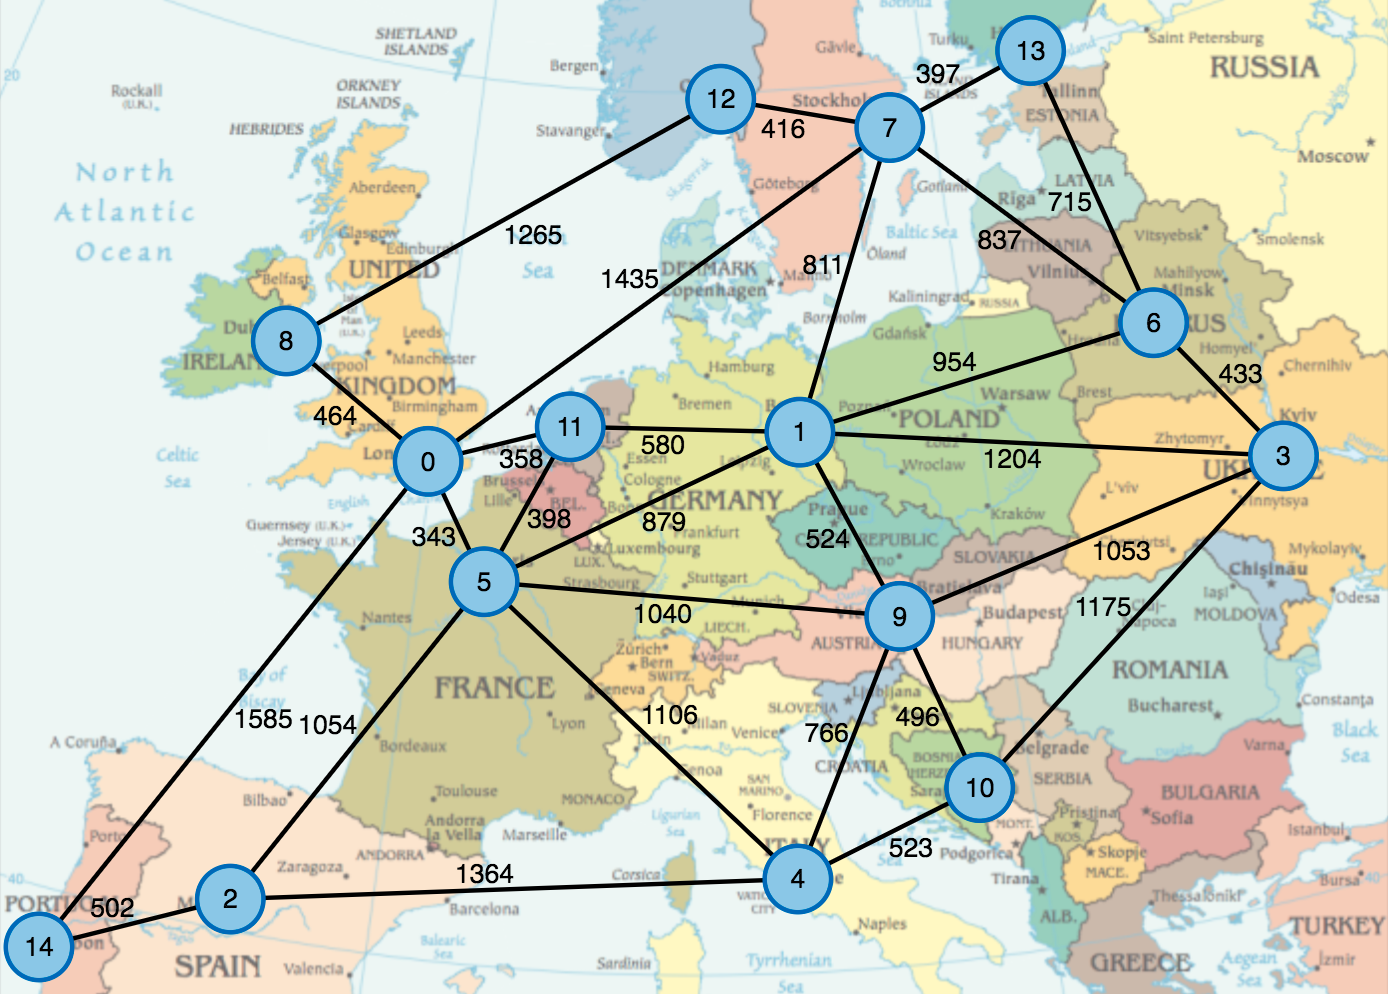
\includegraphics[width=1\linewidth]{slike/gradovi.png}
\caption{Povezivanje europskih gradova}
\label{figmat}
\end{figure}

Kako se graf sastoji od 15 gradova (čvorova) neće biti prikazana svaka iteracija Primovog algoritma, već samo konačno rješenje. Ukoliko je grad Sarajevo (10) označen kao početni čvor, dobija se sljedeće minimalno povezujuće stablo:

\begin{figure}[H]
\centering
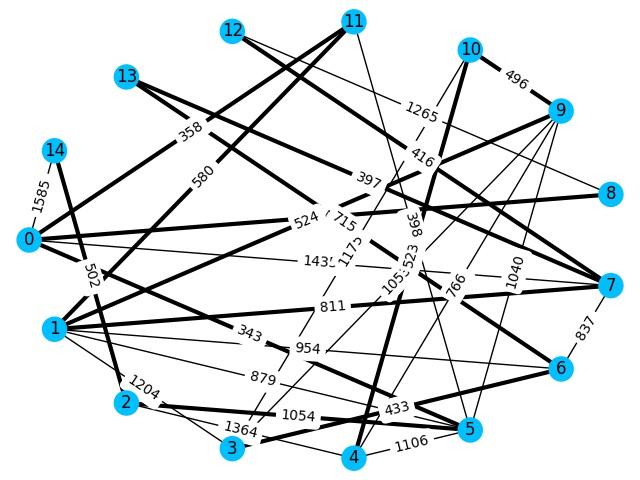
\includegraphics[width=1\linewidth]{slike/gradovi2.jpg}
\caption{MST za europske gradove - Python plot}
\label{figmat}
\end{figure}

\begin{figure}[H]
\centering
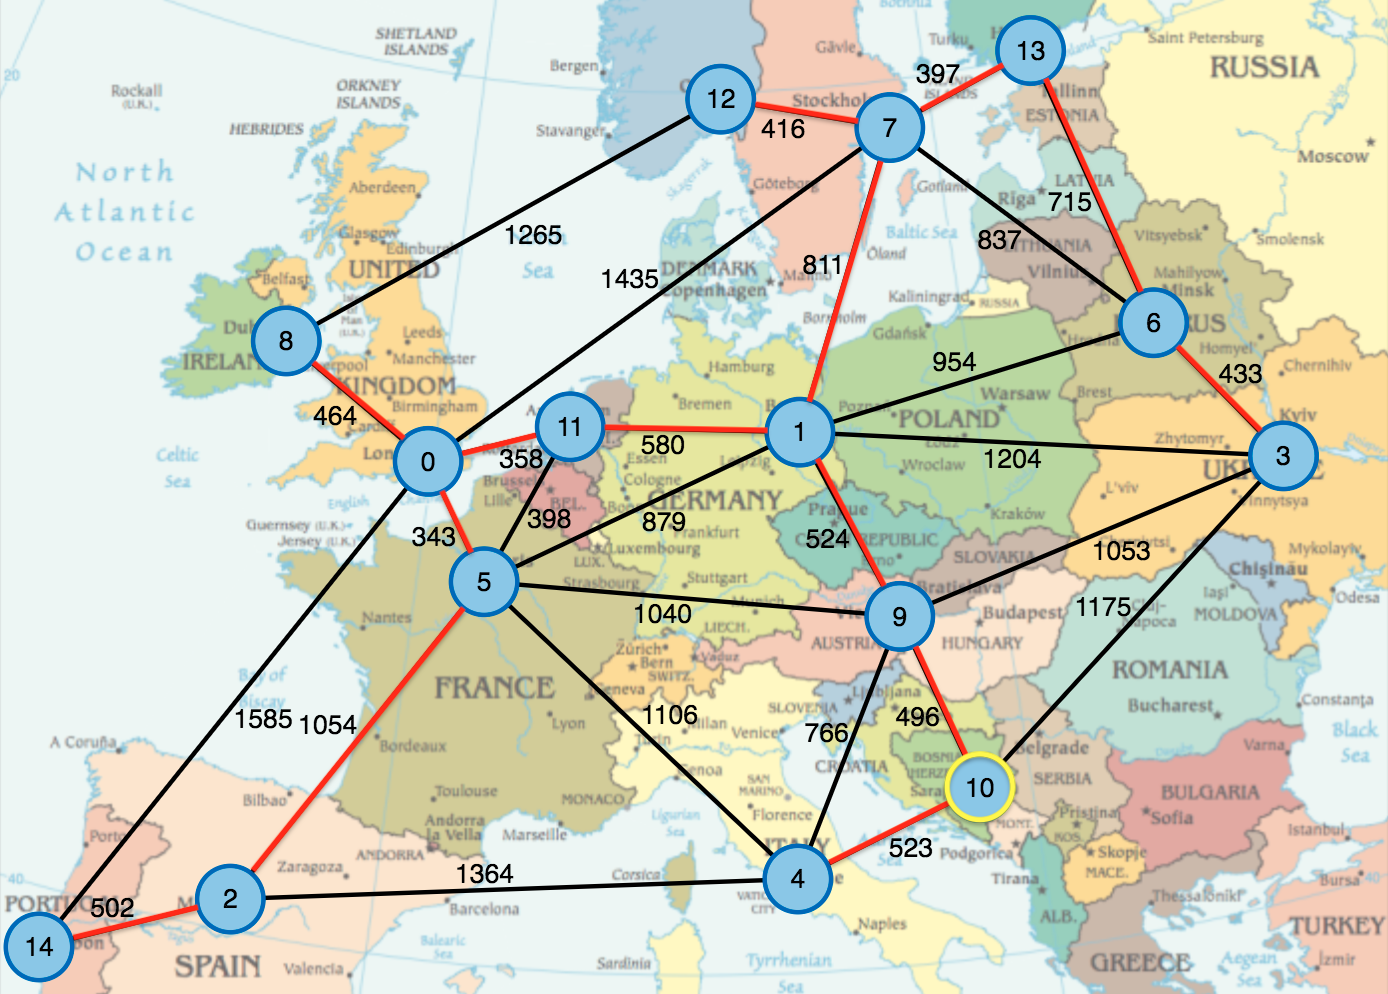
\includegraphics[width=1\linewidth]{slike/gradovi-mst2.png}
\caption{MST za europske gradove}
\label{figmat}
\end{figure}

Kostur je formiran nakon što je izabrano 14 grana (označene crvenom bojom): (Sarajevo - Beč), (Sarajevo - Rim), (Beč - Berlin), (Berlin - Amsterdam), (Amsterdam - London), (London - Pariz), (London - Dablin), (Berlin - Štokholm), (Štokholm - Helsinki), (Štokholm - Oslo), (Helsinki - Minsk), (Minsk - Kiev), (Pariz - Madrid) i (Madrid - Lisabon). Traženo minimalno povezujuće stablo ima ukupnu težinu: 496 + 523 + 524 + 580 + 358 + 343 + 464 + 811 + 397 + 416 + 715 + 433 + 1054 + 502 = 7616. Dakle za povezivanje gradova je potrebno 7616 kilometara optičkog kabla.

Na isti način kao u prethodnom problemu, odredit će se ukupna maksimalna ušteda resursa. U ovom slučaju najveći bi utrošak bio od 14777 kilometara iz čega slijedi je pomoću Primovog algoritma ostvarena ušteda od 7161 kilometara optičkog kabla što je procentualno ($\sim48\%$) uštede.


\subsection{Performanse implementiranog algoritma}

U ovom potpoglavlju je izvršeno testiranje performansi implementiranog Primovog algoritma nad različitim veličinama potpuno gustih grafova.

\begin{figure}[H]
\centering
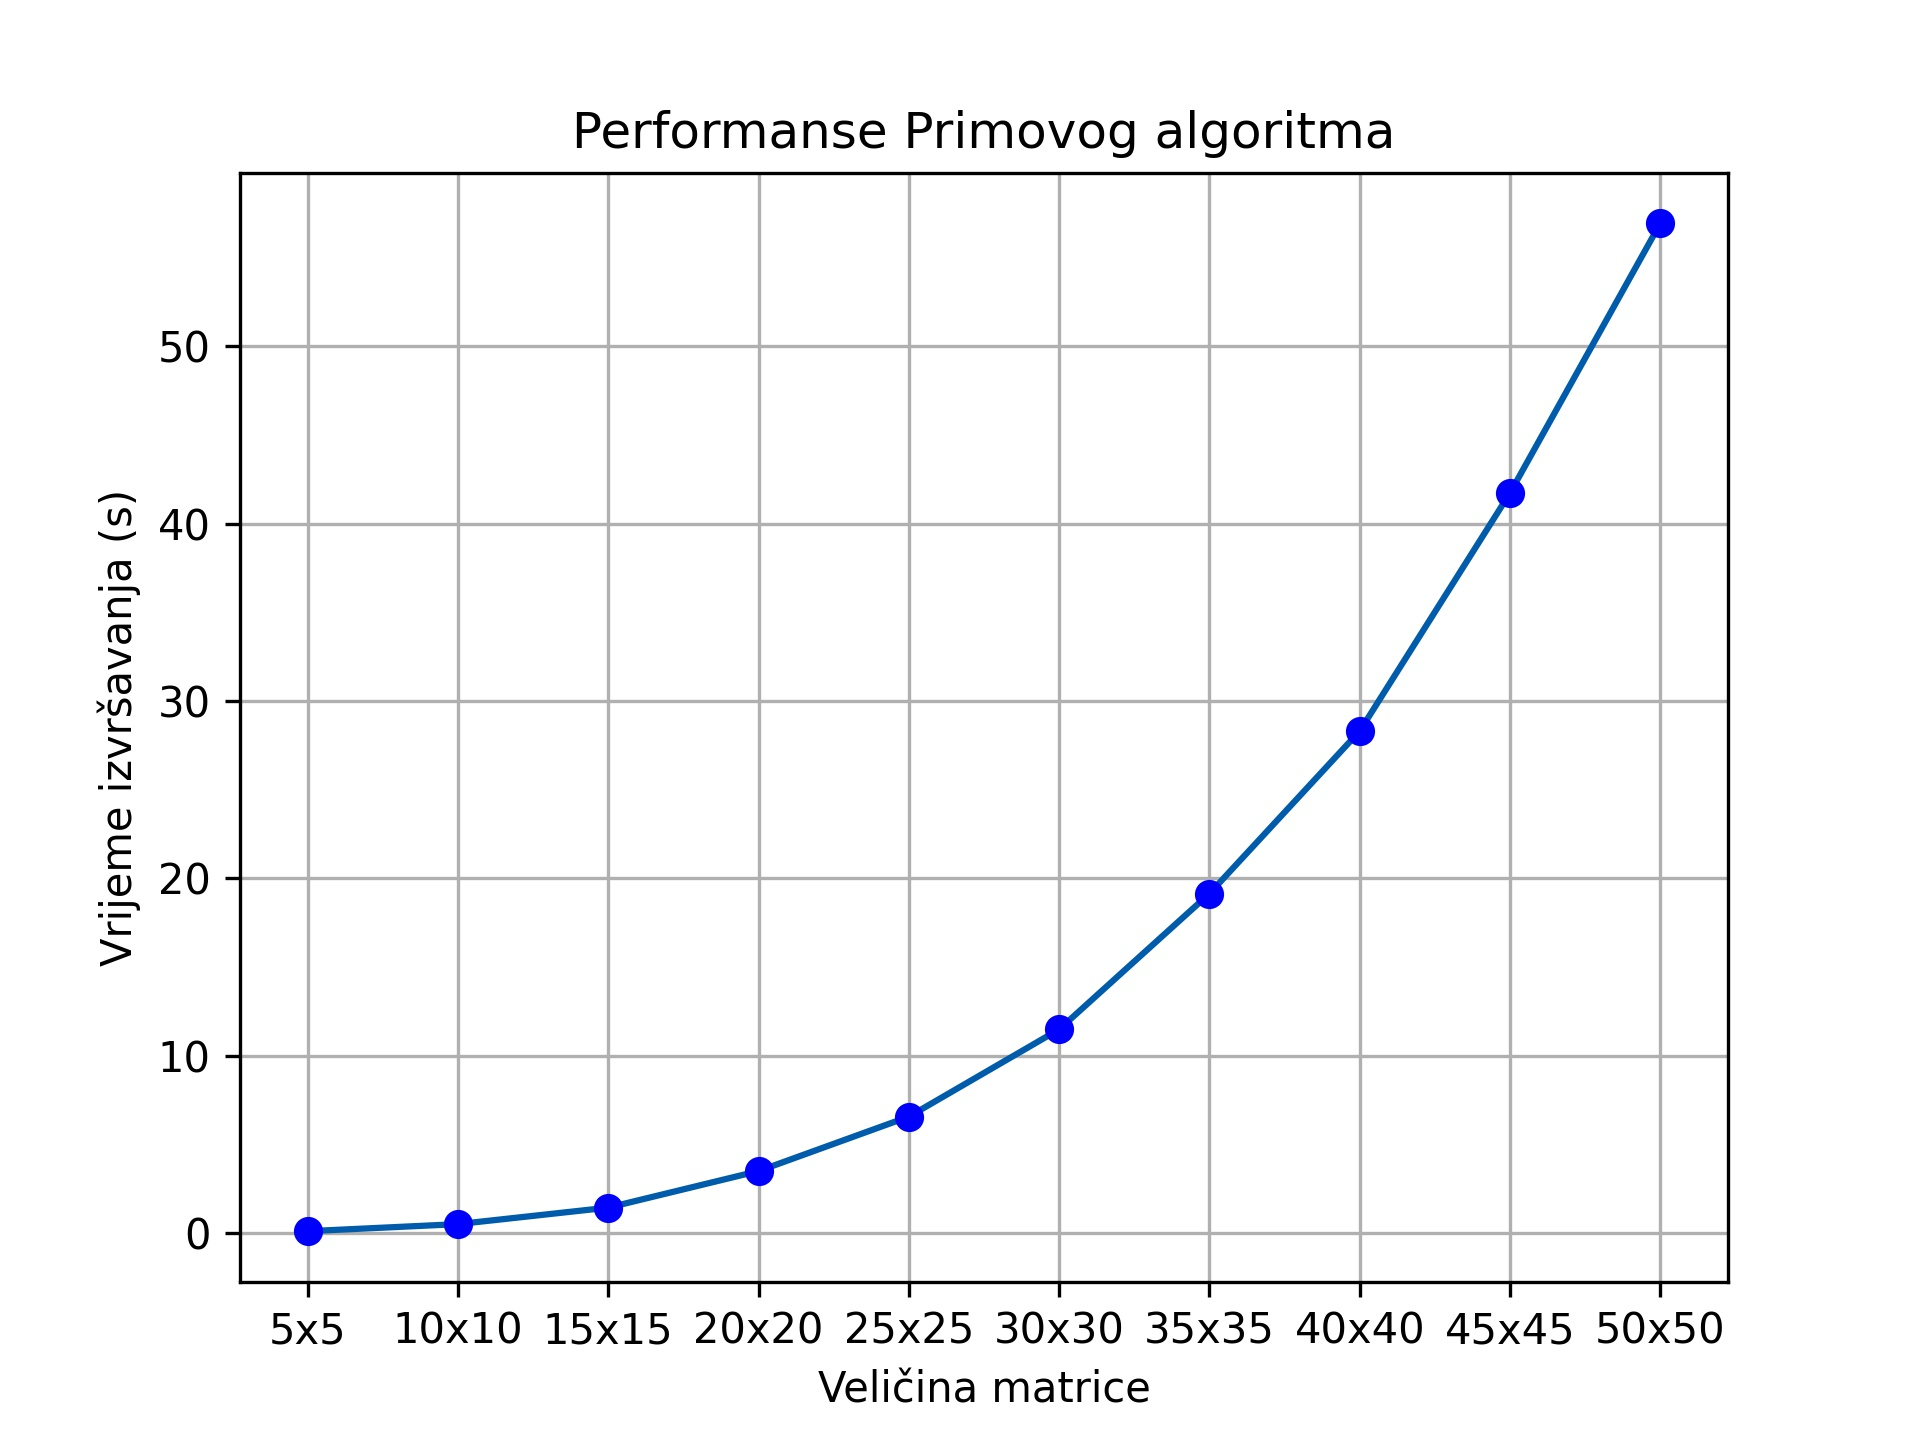
\includegraphics[width=1\linewidth]{slike/performanse/prim-300dpi.jpg}
\caption{Prosječno vrijeme izvršavanja Primovog algoritma za različite veličine potpuno gustih grafova}
\label{figmat}
\end{figure}

Na $x$ osi je predstavljeno prosječno vrijeme izvršavanja, a na $y$ osi veličina matrice susjedstva. Testiranje je izvršeno nad veličinama od 5×5 do 50×50, gdje se u svakom koraku veličina povećava za 5.

Kao rezultat testiranja, dobijena je funkcija za eksponencijalnim rastom. Ova verzija Primovog algoritma za pronalaženje minimalnog povezujućeg stabla nad gustim grafovima dimenzija većih od 50×50 zahtjeva više od 1 minute. Eksponencijalni rast je očekivan s obzirom da se radi o osnovnoj verziji Primovog algoritma.


\section{Zaključak}
Problem rješavanja minimalnog povezujućeg stabla predstavlja jedan od najpopularnijih i najstarijih problema teorije grafova koji ima svoju prepoznatljivu i široku primjenu u praksi. Rješavanjem ovog problema se uspješno pronalazi lista relacija koje je neophodno oformiti među objektima problemskog prostora da bi se ostvario minimalni utrošak resursa što rezultira postizanjem potrebnih ušteda.

Generalno za problem rješavanja minimalnog povezujućeg stabla postoji cijeli spektar metoda i algoritama koji omogućavaju uspješno rješavanjeg istog. Treba također imati u vidu da iako su razvijeni efikasni algoritmi, oni ne mogu imati optimalne performanse za grafove različitih gustoća. Tako da se primjena istih treba prilagoditi u skladu s gustoćom razmatranog grafa. Za implementacionu fazu je odabrana osnovna verzija Primovog algoritma koja je kroz simulacije dala optimalne rezultate. Osim Primovog algoritma, ostali često korišteni algoritmi iz ove oblasti su opisani u kratkim crtama.

Zadatak ovog rada je bila da se odabrani algoritam implementira u programskom jeziku Python i obavi detaljna analiza principa rada istog.
Ova verzija Primovog algoritma relativno brzo pronalazi rješenje za grafove manje gustoće, međutim kako raste gustoća grafa tako vrijeme izvršenja postaje lošije i doseže eksponencijalne nivoe. Da bi se obavio proces simuliranja ovog algoritma osmišljena su dva praktična problema; problem povezivanja dalekovoda i problem povezivanja gradova optičkim kablom.
Primjenom ovog algoritma nad praktičnim problemima  je zamjećena značajna ušteda ($\sim50\%$ za oba problema) što je i osnovni cilj ovog algoritma. Osim osnovne verzije Primovog algoritma postoje i poboljšane verzije koje koriste drugačije pristupe nalaženja grana najmanje težine.Jedan od često korištenih pristupa je korištenje prioritetnog reda. Ovaj pristup, odnosno način implementacije bi mogao smanjiti kompleknost algoritma na $\mathcal{O}(E\log_2 V)$ \cite{b2} i samim time imati bolje performanse nad većim gustim grafovima.





\begin{thebibliography}{00}
\bibitem{b1} Željko Jurić, Predavanja na predmetu Diskretna matematika, Elektrotehnički fakultet, Univerzitet u Sarajevu, ak. 2020/2021. godina.

\bibitem{b2} Haris Šupić, Predavanja na predmetu Algoritmi i strukture podataka, Elektrotehnički fakultet, Univerzitet u Sarajevu, ak. 2020/2021. godina.

\bibitem{b3} Marpaung, F \& Piliang, Arnita. (2020). Comparative of prim’s and boruvka’s algorithm to solve minimum spanning tree problems. Journal of Physics: Conference Series. 1462. 012043. 10.1088/1742-6596/1462/1/012043. 

\bibitem{b4} Tadej Mateljan, Željko Jurić, Predavanja na predmetu Osnove operacionih istraživanja, Elektrotehnički fakultet, Univerzitet u Sarajevu, ak. 2020/2021. godina.


\end{thebibliography}


\end{document}
